\documentclass[a4paper,10pt]{article}
\usepackage[utf8]{inputenc}

% ----  Useful packages % ---- 
\usepackage{amsmath}
\usepackage{graphicx}
\usepackage{amsfonts}
\usepackage{amsthm}
\usepackage{amssymb}
\usepackage{makecell}
\usepackage{tikz}
\usetikzlibrary{arrows.meta}
% ----  Useful packages % ---- 

\usepackage{pythonhighlight}
\usepackage{wrapfig}
\usepackage{caption}
\usepackage{subcaption}
\usepackage{hyperref}
\hypersetup{
	colorlinks,
	citecolor=black,
	filecolor=black,
	linkcolor=black,
	urlcolor=black
}

% ---- Set page size and margins replace ------
\usepackage[letterpaper,top=2cm,bottom=2cm,left=3cm,right=3cm,marginparwidth=1.75cm]{geometry}
% ---- Set page size and margins replace ------

% ------- NOTA ------
\theoremstyle{remark}
\newtheorem{note}{Note}[subsection]
% ------- NOTA ------

% ------- OSSERVAZIONE ------
\theoremstyle{definition}
\newtheorem{observation}{Osservazione}[subsection]
% ------- OSSERVAZIONE ------

% ------- DEFINIZIONE ------
\theoremstyle{plain}
\newtheorem{definition}{Definizione}[subsection]
% ------- DEFINIZIONE ------

% ------- ESEMPIO ------
\theoremstyle{definition}
\newtheorem{example}{Esempio}[subsection]
% ------- ESEMPIO ------

% ------- DIMOSTRAZIONE ------
\theoremstyle{definition}
\newtheorem{demostration}{Dimotrazione}[subsection]
% ------- DIMOSTRAZIONE ------

% ------- TEOREMA ------
\theoremstyle{definition}
\newtheorem{theorem}{Teorema}[subsection]
% ------- TEOREMA ------

% ------- COROLLARIO ------
\theoremstyle{plain}
\newtheorem{corollaries}{Corollario}[theorem]
% ------- COROLLARIO ------

% ------- PROPOSIZIONE ------
\theoremstyle{plain}
\newtheorem{proposition}{Proposizione}[subsection]
% ------- PROPOSIZIONE ------

% ---- Footer and header ---- 
\usepackage{fancyhdr}
\pagestyle{fancy}
\fancyhf{}
\fancyhead[LE,RO]{A.A 2023-2024}
\fancyhead[RE,LO]{Introduzione all'intelligenza artificiale}
\fancyfoot[RE,LO]{\rightmark}
\fancyfoot[LE,RO]{\thepage}

\renewcommand{\headrulewidth}{.5pt}
\renewcommand{\footrulewidth}{.5pt}
% ---- Footer and header ---- 

% ----  Language setting ---- 
\usepackage[italian, english]{babel}
% ----  Language setting ---- 

\usepackage{listings}
\usepackage{color}

\definecolor{dkgreen}{rgb}{0,0.6,0}
\definecolor{gray}{rgb}{0.5,0.5,0.5}
\definecolor{mauve}{rgb}{0.58,0,0.82}

\lstset{frame=tb,
	language=C,
	aboveskip=3mm,
	belowskip=3mm,
	showstringspaces=false,
	columns=flexible,
	basicstyle={\small\ttfamily},
	numbers=none,
	numberstyle=\tiny\color{gray},
	keywordstyle=\color{blue},
	commentstyle=\color{dkgreen},
	stringstyle=\color{mauve},
	breaklines=true,
	breakatwhitespace=true,
	tabsize=3
}

\title{\textbf{Introduzione all'Intelligenza Artificiale}}
\author{Realizzato da: Matteo Giuntoni, Ghirardini Filippo}
\date{A.A. 2023-2024}

\begin{document}
	\begin{titlepage} %crea l'enviroment
	\begin{figure}[t] %inserisce le figure
		\centering
\includegraphics[width=0.98\textwidth]{marchio_unipi_pant541.png}
	\end{figure}
	\vspace{20mm}
	
	\begin{Large}
		\begin{center}
			\textbf{Dipartimento di Informatica\\ Corso di Laurea Triennale in Informatica\\}
			\vspace{20mm}
			{\LARGE{Corso a Libera Scelta - 6 CFU}}\\
			\vspace{10mm}
			{\huge{\bf Computer Graphics}}\\
		\end{center}
	\end{Large}
	
	
	\vspace{36mm}
	%minipage divide la pagina in due sezioni settabili
	\begin{minipage}[t]{0.47\textwidth}
		{\large{\bf Professore:}\\ \large{Prof. }}
	\end{minipage}
	\hfill
	\begin{minipage}[t]{0.47\textwidth}\raggedleft
		{\large{\bf Autore:}\\ \large{Filippo Ghirardini}}
	\end{minipage}
	
	\vspace{25mm}
	
	\hrulefill
	
	\vspace{5mm}
	
	\centering{\large{\bf Anno Accademico 2023/2024 }}
	
\end{titlepage}
	
	\tableofcontents
	\newpage
	\maketitle
	\begin{center}
		\vspace{-20pt}
		\rule{11cm}{.1pt} 
	\end{center}
	\section{Punto materiale}
Oggetto caratterizzato da una massa [kg] e da un vettore posizione [m] nello spazio 3D.
Dimensioni trascurabili, forma irrilevante rispetto ai fenomeni di interesse.
Vettore posizione come funzione del tempo t[s].
\begin{example}
    Una molecola di ossigeno se sono interessato all'aereodinamica di una vettua. 
    Un satellite attorno alla terra se ignoro le forze di marea.
\end{example}
\hspace{-15pt}\textbf{Un vettore posizione} è una funzione del tempo $t[s]$.
$$\vec{r(t)} = (x(t), y(t), z(t)) = x(t)\hat{x} + y(t)\hat{z} + z(t)\hat{z}$$
\begin{observation}
    I versori cartesiani sono costanti
\end{observation}

\begin{definition}[Legge oraria]
    Si definisce come legge oraria la funzione $t \mapsto \vec{r}(t)$.
\end{definition}

\begin{definition}[Traiettoria]
    Il luogo geometrico di punti visitati dal punto materiale.
    $$\{\vec{r}(t)\:\: per \: t \in \mathbb{R}\}$$
\end{definition}

\begin{example}
    $\vec{r}(t) = (v_0t, y_0, 0)$ e $v_0 = 3m/s, y_o = 5m$ 
    \begin{figure}[h!]
        \centering
        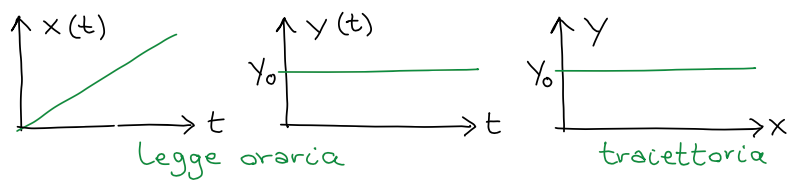
\includegraphics[width=0.8\textwidth]{images/ess-traiettoria.png}
    \end{figure}
\end{example}

\begin{definition}
    La \textbf{velocità istantanea} è la derivata della posizione rispetto al tempo.
    $$v = \lim_{\Delta t \to 0}\frac{\Delta s}{\Delta t} = \frac{ds}{dt}$$
\end{definition}

\begin{definition}
    La \textbf{velocità media} è definita come il rapporto tra lo spostamento e l'intervallo di tempo necessario per effettuarlo.
    $$v_m = \frac{\Delta s}{\Delta t}$$
\end{definition}
\hspace{-15pt}In parole povere è una grandezza che ci dice con quale rapidità cambia la posizione di un punto rispetto al tempo nell'instante $t$.
\subsection*{Vettore velocità}
Derivata rispetto al tempo del vettore posizione e si indica come 
$\frac{d\vec{r}(t)}{dt}\text{ oppure }\dot{\vec{r}}(t)[m/s]$
\begin{equation}
    \begin{split}
    \dot{\vec{r}}(t) & = (\dot{x}(t), \dot{y}(t), \dot{z}(t)) \\
     & = \frac{d}{dt}[x(t)\hat{x} + y(t)\hat{y} + z(t)\hat{z}] \\
     & = \dot{x}(t)\hat{x} + \dot{y}(t)\hat{y} + \dot{z}(t)\hat{z}
    \end{split}
\end{equation}
Per ricavare la forma esplicita uso le proprietà delle derivate (\textbf{linearità}, \textbf{Leibnitz})
\begin{example}
    $\vec{r}(t) = (v_0t, y_0, 0) = v_0t\hat{x} + y_0\hat{y}$ \:\:\:abbiamo che \:\:\:
    $\dot{\vec{r}}(t) = (v_0, 0, 0) = v_0 \hat{x}$
\end{example}
\hspace{-15pt}Velocità e spazio percorso ("integrale di linea").\\
\begin{wrapfigure}[3]{l}{5cm}
    \centering
    \includegraphics[width=5cm]{images/vettore-velocità.png}
\end{wrapfigure}
\begin{align*}
    L & = ||\vec{r}(t_1) - \vec{r}(t_0)|| + ||\vec{r}(t_2) - \vec{r}(t_1)|| + ||\vec{r}(t_3) - \vec{r}(t_2)|| + \dots \\
    & = \sum_i ||\vec{r}(t_{i+1} - \vec{r}(t_i)|| \:\: per\:\: |t_{i+1} - t_i| \text{"piccolo"} \\
    & = \sum_i ||\frac{\vec{r}(t_{i+1}) - \vec{r}(t_i)}{t_{i+1} - t_i}|| (t_{i+1} - t_i) = \int_{t_{in}}^{t_{f_{in}}}||\dot{\vec{r}}(t)||\\
\end{align*}
\begin{example}
    $\vec{r}(t) = (v_0t, y_0)\:\:\: \dot{\vec{r}}(t) = (v_0, 0)$\hspace{15pt}
    $||\dot{\vec{r}}(t)|| = \sqrt{v_0^2 + 0^2} = |v_0|$ \:\:\: $L = |v_0| \cdot (t_{f_{in}} - t_{in})$\\
    Il vettore è costante quindi facendo la derivata torna zero. Con la velocità si calcolo lo spazio percorso ("integrale di linea").
    La differenza fra le posizioni e la differenza dei tempi è il rapporto incrementale in caso gli intervalli siano sufficentemente
    piccoli, da qui si ottiene l'integrale.
\end{example}

\subsection{Vettore accelerazione}
Derivata rispetto al tempo del vettore velocità e si indica con $\frac{d^2\vec{r}(t)}{dt} \text{ oppure } \ddot{\vec{r}}(t) [m/s^2]$
\begin{equation}
    \ddot{\vec{r}}(t) = (\ddot{x}(t), \ddot{y}(t), \ddot{z}(t))\:\: = \:\: \ddot{x}(t)\hat{x} + \ddot{y}(t)\hat{y} + \ddot{z}(t)\hat{z}
\end{equation}
\begin{example}
    $\vec{r}(t)= (\frac{1}{2}a_0t^2, v_0t, 0)$ \hspace{10pt} $\dot{\vec{r}}(t) = (a_0t, v_0, 0)$ \hspace{10pt} $\dot{\vec{r}}(t) = (a_0, 0, 0)$
\end{example}
\hspace{-15pt}Serve perché l'equazione "del moto" di Newton che determinata la legge oraria è formulata in termini di accelerazione.

\subsection{Vettore quantità di moto}
Il prodotto di massa [kg] e velocità [m/s]
$$\vec{p}(t) = m \cdot \dot{\vec{r}}(t) = (m\dot{x}(t), m\dot{y}(t), m\dot{x}(t)) = m\dot{\vec{x}}(t)x + m\dot{\vec{y}}(t)y + m \dot{\vec{z}}(t)z$$
\begin{example}
    Prendiamo un punto di massa 2kg e velocità 3m/s lungo $\hat{x}$.\\
    $p_x(t) = 2 \cdot 3 kg\cdot m/s = 6 kg \cdot m/s$ \hspace{15pt} $p_y(t) = p_z(t) = 0$.
\end{example}
\hspace{-15pt}Serve per generalizzare l'equazione di Newton e per trattare sistemi di piu punti materiali.

\subsection{Vettore momento angolare rispetto a un polo P}
$$\vec{L}_p(t) = m(\vec{r}(t) - \vec{r}_p) \times \dot{\vec{r}}(t)$$
Dove $\vec{r}_p$ è il vettore posizione di p, mentre $\dot{\vec{r}}(t)$ è il prodotto vettoriale.
\begin{example}
    $\vec{r}_p = (l_0, 0, 0)$ \hspace{15pt} $\vec{r}(t) = (v_0t, y_0, 0)$\\
    $\vec{L}_p = m[(v_0t - l_0)\hat{x} + y_0\hat{y}] \times (v_0\hat{x}) \:\: = \:\: m(v_0t - l_0)v_0 \hat{x} \times \hat{x} + my_0v_0\hat{y}\times \hat{x} 
    \:\: = \:\: my_0v_0(-\hat{z}) = (0,0, -my_0v_0)$\\
    Ricorda che $\hat{x} \times \hat{x} = 0$ e $\hat{y} \times \hat{x} = -\hat{z}$
\end{example}
\hspace{-15pt}Il momento angolare dice quanta inerzia ha un oggetto in una rotazione (descrizione sommaria).\\
Il polo P è parte della definizione. È una scelta! Il risultato dipende dal polo.
Serve per formulare l'equazione del moto di sistemi di punti materiali e corpi rigidi.

\subsection{Coordinate polari}
Un metodo per rapprensentare delle cordinate x, y andando a misurare prima la distanza dall'origine e poi si va a vedere
quanto vale l'angolo fra questo segmento dall'asse x, utilizzando seno e coseno.
\begin{wrapfigure}[7]{l}{2cm}
    \centering
    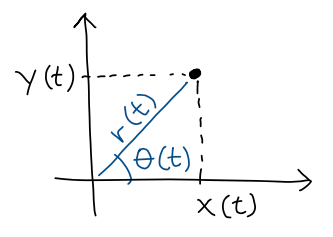
\includegraphics[width=5.5cm]{images/coordinate-polari.png}
\end{wrapfigure}
\begin{align*}
    \begin{cases}
        x(t) = r(t) \cdot \cos(\Theta(t))\\
        y(t) = r(t) \cdot \sin(\Theta(t)) 
    \end{cases}
\end{align*}
\begin{align*}
    \begin{cases}
        r(t) = \sqrt{x(t)^2 + y(t)^2} \geq 0\\
        tg(\Theta(t)) = y(t) / x(t) 
    \end{cases}
\end{align*}
\\
\begin{example} Esempi di rappresentazione di coordinate in coordinate polari.\\
    $x = 0, y = l_0 > 0 \:\: \Rightarrow \:\: r = l_0, \Theta = \pi/2$\\
    $x = 0, y = -l_0 < 0 \:\: \Rightarrow \:\: r = l_0, \Theta = -\pi/2$\\
    $x = l_0, y = l_0 > 0 \:\: \Rightarrow \:\: r = \sqrt{2}l_0, \Theta = \pi/4$\\
\end{example}

\subsection{Versori polari (2D)}
Definisco un versore $\hat{r}(t)$ che punta verso il punto materiale e un versore $\hat{\Theta}(t)$ ortogonale.
Si esprime facilmente in coordinte polari.
$$\vec{r}(t) = (x(t), y(t)) = (r(t)\cos \Theta(t), r(t)\sin\Theta(t)) \:\: = \:\: r(t)(\cos\Theta(t)\hat{x} + \sin\Theta(t)\hat{y})$$
Ma $||\vec{r}(t)|| = |r(t)| = r(t)$ allora definisco $\hat{r}(t) = \vec{r}(t)/ ||\vec{r}(t)|| = \cos \Theta(t)\hat{x} + \sin\Theta(t)\hat{y}$\\\\
Trovo facilmente che un versore ortogonale è:
$$\hat{\Theta(t)} = -\sin\Theta(t)\hat{x} + \cos\Theta(t)\hat{y} \:\:\:\text{infatti} \:\:\: \hat{r}\cdot \hat{\Theta} = c \cdot (-s) + s \cdot c = 0$$
\begin{wrapfigure}[7]{r}{6cm}
    \centering
    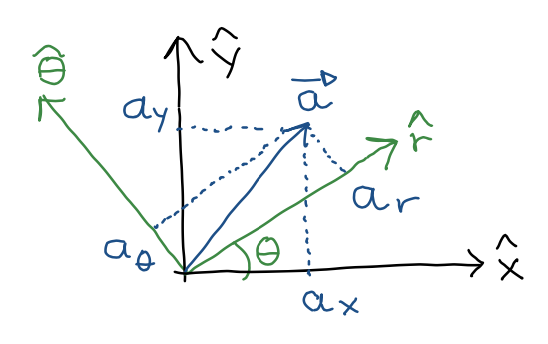
\includegraphics[width=5.5cm]{images/trasformazioni-inverse.png}
\end{wrapfigure}
\begin{note}
    Non c'è legame fra $\Theta$ e $\hat{\Theta}$ è solo una convenzione.
\end{note}
\hspace{-15pt}Le trasformazioni inverse invece si fanno come segue (verifico per sostituzione):
$$\hat{y} = \cos\Theta(t)\hat{r} - \sin\Theta(t)\hat{\Theta} \hspace{20pt} \hat{y} = \sin\Theta(t)\hat{r} + \cos\Theta(t)\hat{\Theta}$$
Possono quindi scrivere ogni vettore nella forma $\vec{a} = a_r\hat{r} + a_{\Theta}\hat{\Theta}$ con le componenti polari $a_r, a_{\Theta}$.
Per evitare ambiguità non scriviamo $(a_r, a_{\Theta})$ e riserviamo la notazione alle componenti cartesiane.\\\\
A differenza dei versori cartesiani quelli polari dipendono dal tempo per costruzioni.
$$\dot{\hat{r}}(t) = \frac{d}{dt}[\cos\Theta(t) \hat{x} + \sin\Theta(t)\hat{y}] \:\: = \:\: -\sin\Theta(t) \cdot \dot{\Theta}(t)\hat{x} + \cos\Theta(t) \cdot \dot{\Theta}(t)\hat{y}$$
Dove $\cos\Theta(t) \cdot \dot{\Theta}(t)$ si applica la derivata della somma, Leibnitz, funzione composta.
$$= \dot{\Theta}(t)\cdot \hat{\Theta}(t) \:\:\:\:(\text{confronto l'espressione di} \hat{\Theta}(t))$$
Similmente $\dot{\hat{\Theta}}(t)= - \dot{\Theta}\hat{r}(t)$.


\subsection*{Vettori posizione, velocità, accelerazione}
$$\vec{r}(t) = r(t)\hat{r}(t)$$
Dove abbiamo che $\vec{r}(t)$ è il vettore, $r(t)$ è una coordinata polare, $\hat{t}(t)$ è il versore polare.
$$\dot{\vec{r}}(r) = \dot{r}(t)\hat{r}(t) + r(t)\dot{\Theta}(t)\hat{\Theta}(t)$$
Dove la parte $\dot{\vec{r}}(r)$ è la velocità radiale.
$$\ddot{\vec{r}}(t) = [\ddot{r}(t) - r(t)\dot{\Theta}(t)^2] \hat{r} + [r(t) \ddot{\Theta}(t) + 2\dot{r}(t)\dot{\Theta}(t)]\hat{\Theta}$$
Nel quale abbiamo che la parte $r(t)\dot{\Theta}(t)^2$ si chiama \textbf{velocità centripeta}, mentre $2\dot{r}(t)\dot{\Theta}(t)$ si dice \textbf{accelerazione di Coriolis}.


	% !TeX spellcheck = it_IT
\newpage
\section{Agenti intelligenti}
L'approccio moderno dell'IA (AIMA) è quello di costruire degli \textbf{agenti intelligenti}. La visione ad agenti offre n quadro di riferimento e una prospettiva più generale. È utile anche perché è \textbf{uniforme}.
\begin{center}
	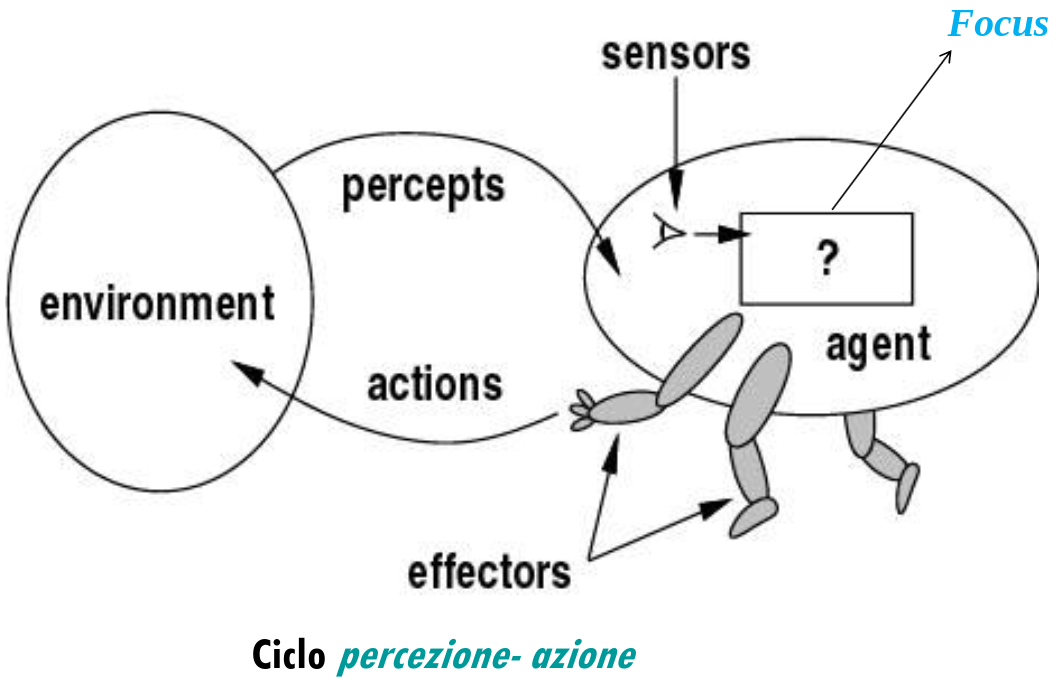
\includegraphics[scale=0.25]{images/agente.png}
\end{center}
Noi ci concentreremo sul programma che sta al centro dell'agente e che consiste in un ciclo di percezione-azione.
\subsection{Caratteristiche}
Un agente ha alcune caratteristiche:
\begin{itemize}
	\item \textbf{Situati}: ricevono \emph{percezioni} da un ambiente e agiscono mediante \textbf{azioni} (attuatori)
	
\end{itemize}

\subsubsection{Percezioni e azioni}
Le percezioni corrispondono agli \textbf{input} dai sensori. La \textbf{sequenza percettiva} sarà la storia completa delle percezioni.\\
La scelta dell'azione è \emph{funzione} unicamente della sequenza percettiva ed è chiamata \textbf{funzione agente}.\\
Il compito dell'IA è costruire il programma agente.
\begin{center}
	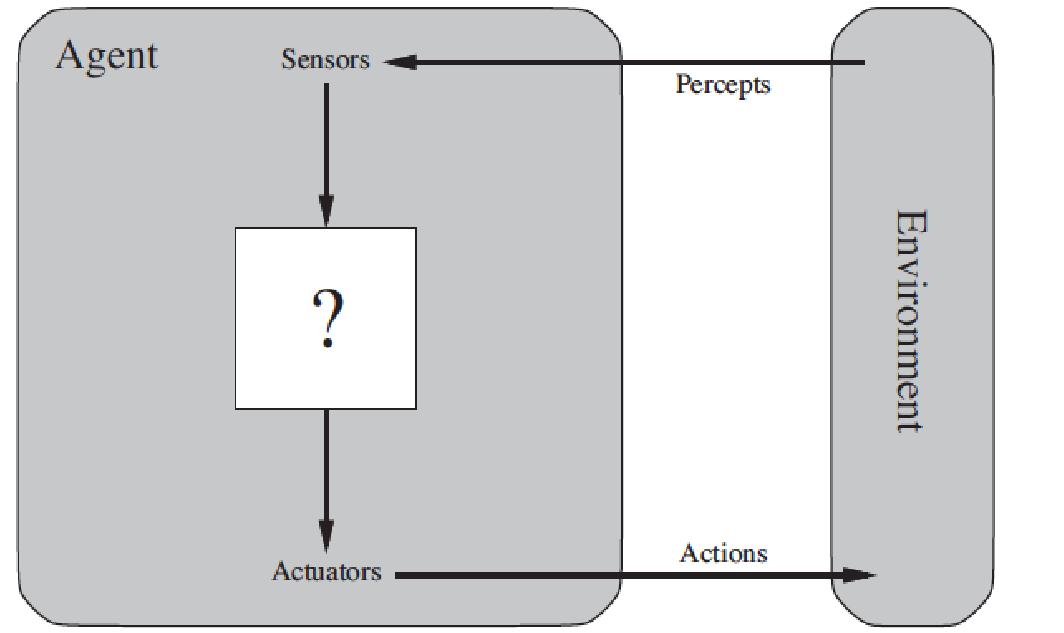
\includegraphics[scale=0.2]{images/architettura_astratta.png}
	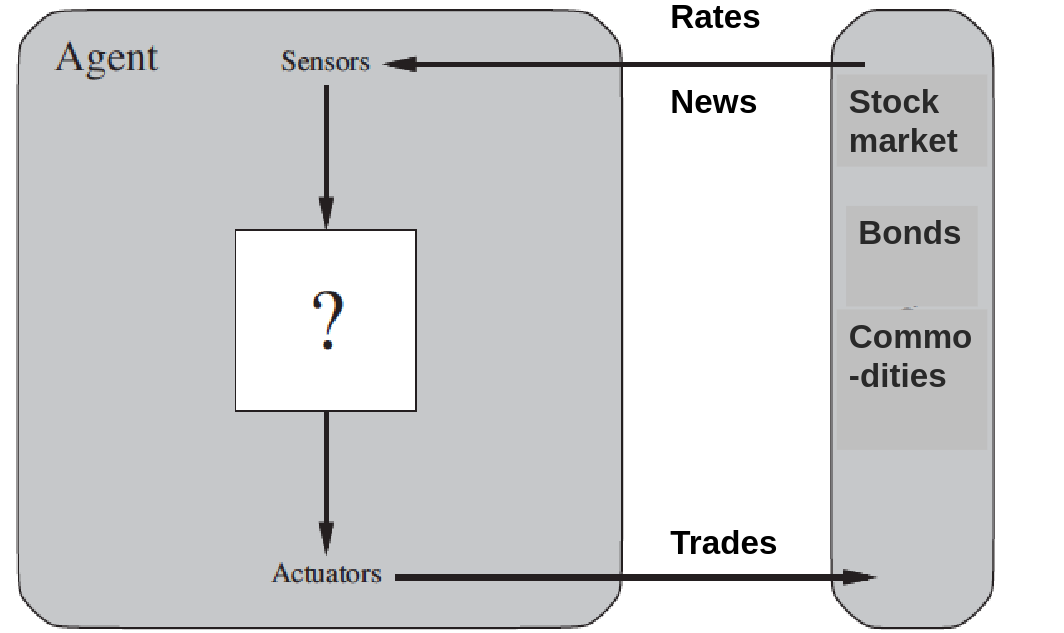
\includegraphics[scale=0.2]{images/agente_finanziario.png}
\end{center}
%TODO Caption

\subsection{Agente razionale}
Un agente razionale interagisce con il suo ambiente in maniera \textbf{efficace} (fa la cosa giusta).
Si rende quindi necessario un \textbf{criterio di valutazione} oggettivo dell'effetto delle azioni dell'agente. La valutazione della prestazione deve avere le seguenti caratteristiche:
\begin{itemize}
	\item Esterna (come vogliamo che il mondo evolva?)
	\item Scelta dal progettista a seconda del problema considerando l'effetto desiderato sull'ambiente.
	\item (possibile) Valutazione su ambienti diversi.
\end{itemize}
\begin{definition}[Agente razionale]
	Per ogni sequenza di percezioni compie l’azione che massimizza il valore atteso della
	misura delle prestazioni, considerando le sue percezioni passate e la sua conoscenza pregressa.
\end{definition}
\begin{observation}
	Si basa sulla razionalità e non sull'onniscenza e onnipotenza: non conosce alla perfezione il futuro ma può apprendere e hai dei limiti nelle sue azioni.
\end{observation}

Raramente tutta la conoscenza sull’ambiente può essere fornita a priori dal programmatore. L’agente razionale deve essere in grado di modificare il proprio comportamento con l’esperienza. Può \textbf{migliorare} esplorando, apprendendo, aumentando l'autonomia per operare in ambienti differenti o mutevoli.

\begin{definition}[Agente autonomo]
	Un agente è autonomo nella misura in cui il suo comportamento dipende dalla sua
	capacità di ottenere esperienza e non dall’aiuto del progettista.
\end{definition}

\subsection{Ambienti}
Definire un problema per un agente significa innanzitutto caratterizzare l'ambiente in cui opera. Viene utilizzata la descrizione \textbf{PEAS}:
\begin{itemize}
	\item \textbf{P}erformance
	\item \textbf{E}nviroment
	\item \textbf{A}ctuators
	\item \textbf{S}ensors
\end{itemize}

\begin{center}
	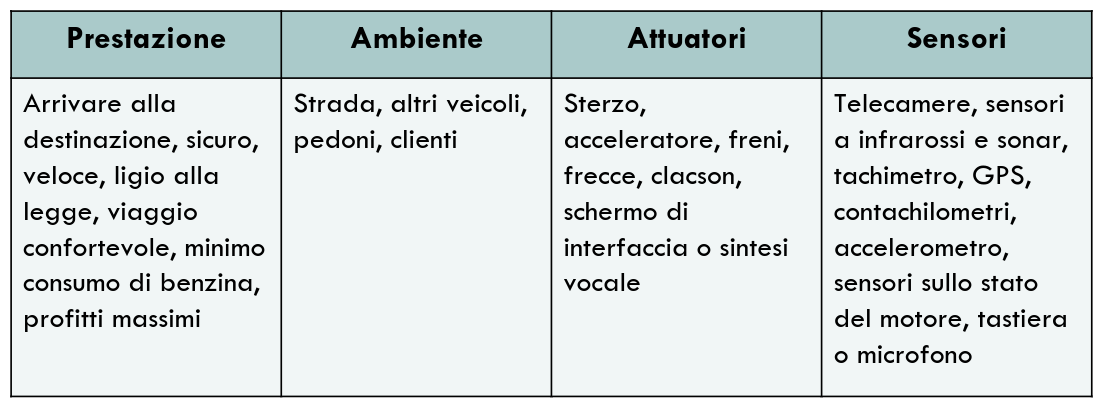
\includegraphics[scale=0.3]{images/agente_ambiente.png}
	%TODO Caption
\end{center}

L'ambiente deve avere le seguenti proprietà:
\begin{itemize}
	\item Osservabilità:
	\begin{itemize}
		\item Se è \textbf{completamente osservabile} l'apparato percettivo è in grado di dare conoscenza completa dell'ambiente o almeno tutto ciò che è necessario per prendere l'azione
		\item Se è \textbf{parzialmente osservabile} sono presenti limiti o inaccuratezze dell'apparato sensoriale
	\end{itemize}
	\item Agente singolo o multi-agente:
	\begin{itemize}
		\item L'ambiente ad agente \textbf{singolo} può anche cambiare per eventi, non
		necessariamente per azioni di agenti
		\item Quello \textbf{multi-agente} può essere \emph{competitivo} (scacchi) o \emph{cooperativo}
	\end{itemize}
	\item Predicibilità:
	\begin{itemize}
		\item \textbf{Deterministico}: quando lo stato successivo è completamente determinato dallo stato corrente e dall’azione (e.g. scacchi)
		\item \textbf{Stocastico}: quando esistono elementi di incertezza con associata probabilità (e.g. guida)
		\item \textbf{Non deterministico}: quando si tiene traccia di più stati possibili risultato dell’azione ma non in base ad una probabilità
	\end{itemize}
\end{itemize}
\newpage
\begin{itemize}
	\item Episodico o sequenziale:
	\begin{itemize}
		\item \textbf{Episodico}: quando l’esperienza dell’agente è divisa in episodi atomici
		indipendenti in cui non c'è bisogno di pianificare (e.g. partite diverse)
		\item \textbf{Sequenziale}: quando ogni decisione influenza le successive (e.g. mosse di scacchi)
	\end{itemize}
	\item Statico o dinamico:
	\begin{itemize}
		\item \textbf{Statico}: il mondo non cambia mentre l’agente decide l’azione (e.g cruciverba)
		\item \textbf{Dinamico}: cambia nel tempo, va osservata la contingenza e tardare equivale a non agire (e.g. taxi)
		\item \textbf{Semi-dinamico}: l’ambiente non cambia ma la valutazione dell’agente sì (e.g. scacchi con timer)
	\end{itemize}
	\item Valori come lo stato, il tempo, le percezioni e le azioni possono assumere valori \textbf{discreti} o \textbf{continui}. Il problema è combinatoriale nel discreto o infinito nel continuo.
	\item \textbf{Noto} o \textbf{ignoto}: una distinzione riferita alla conoscenza dell'agente sulle leggi fisiche dell'ambiente (le regole del gioco). È diverso da osservabile.
\end{itemize}

\begin{definition}[Simulatore]
	Un simulatore è uno strumento software che si occupa di:
	\begin{itemize}
		\item Generare stimoli
		\item Raccogliere le azioni in risposta
		\item Aggiornare lo stato
		\item Attivare altri processi che influenzano l'ambiente
		\item Valutare la prestazione degli agenti (media su più istanze)
	\end{itemize}
	Gli esperimenti su classi di ambienti con condizioni variabili sono essenziali per \textbf{generalizzare}.
\end{definition}

\subsection{Programma agente}
L'agente sarà quindi composto da un'architettura e da un programma. Il programma dell'agente implementa la funzione agente $Ag: Percezioni \to Azioni$. 

\begin{lstlisting}
	function Skeleton-Agent (percept) returns action
		static: memory, agent memory of the world
		memory <- UpdateMemory(memory, percept)
		action <- Choose-Best-Action(memory)
		memory <- UpdateMemory(memory, action)
		return action
\end{lstlisting}

\subsubsection{Tabella}
Un agente basato su tabella esegue una scelta come un accesso ad una tabella che associa un'azione ad ogni possibile sequenza di percezioni.\\
Ha una \textbf{dimensione ingestibile}, è difficile da costruire, non è autonomo ed è di difficile aggiornamento (apprendimento complesso).

\subsubsection{Agenti reattivi}
L'agente agisce in base a quello che percepisce senza salvare nulla in memoria.
\begin{center}
	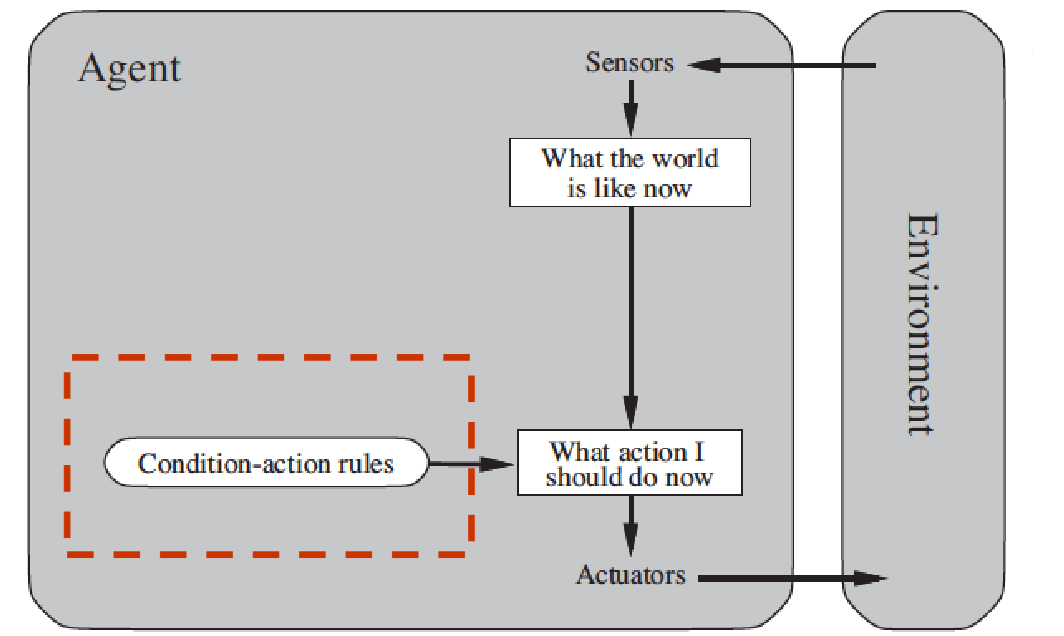
\includegraphics[scale=0.25]{images/agenti_reattivi.png}
\end{center}
\begin{lstlisting}
	function Agente-Reattivo-Semplice (percezione)
		returns azione
		persistent: regole, un insieme di regole
		condizione-azione (if-then)
		stato <- Interpreta-Input(percezione)
		regola <- Regola-Corrispondente(stato, regole)
		azione <- regola.Azione
		return azione
\end{lstlisting}

\subsubsection{Agenti basati su modello}
L'agente ha uno stato che mantiene la storia delle percezioni e influenza il modello del mondo.
\begin{center}
	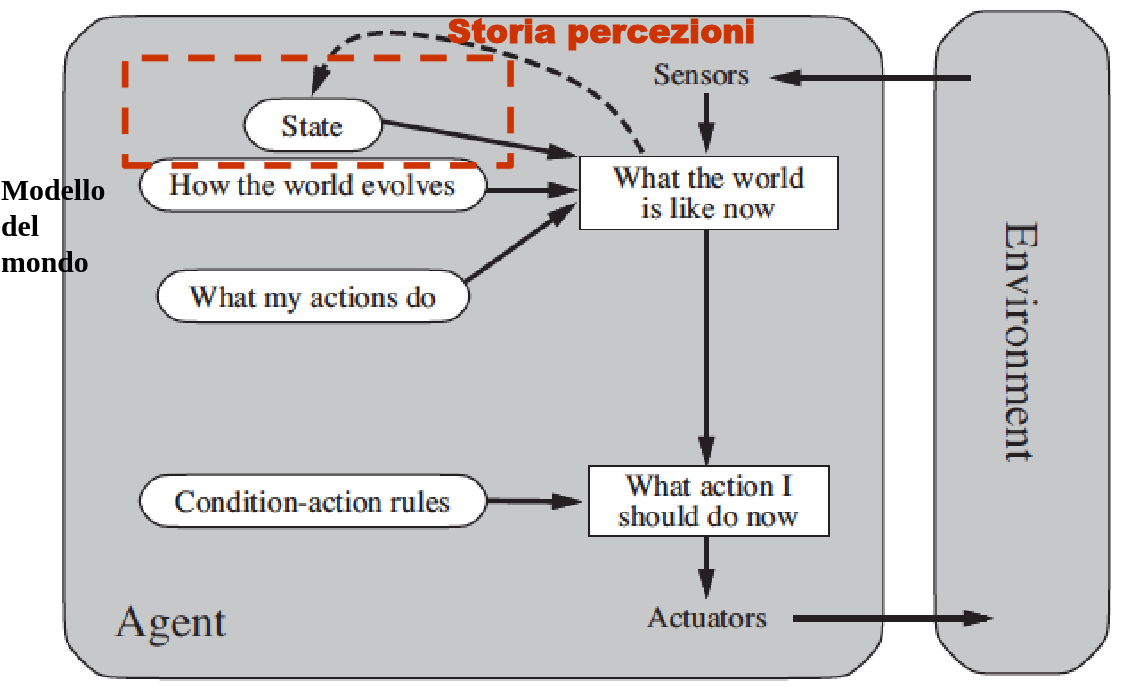
\includegraphics[scale=0.25]{images/agenti_modello.png}
\end{center}
\begin{lstlisting}
	function Agente-Basato-su-Modello (percezione)
		returns azione
		persistent: stato, una descrizione dello stato corrente
								modello, conoscenza del mondo
								regole, un insieme di regole condizione-azione
								azione, azione piu recente
		stato <- Aggiorna-Stato(stato, azione, percez., modello)
		regola <- Regola-Corrispondente(stato, regole)
		azione <- regola.Azione
		return azione
\end{lstlisting}

\subsubsection{Agenti con obiettivo}
Fin'ora l'agente aveva un obiettivo predeterminato dal programma. In questo caso invece viene specificato anche il \textbf{goal} che influenza le azioni. Abbiamo quindi più \textbf{flessibilità} ma meno efficienza.
\begin{center}
	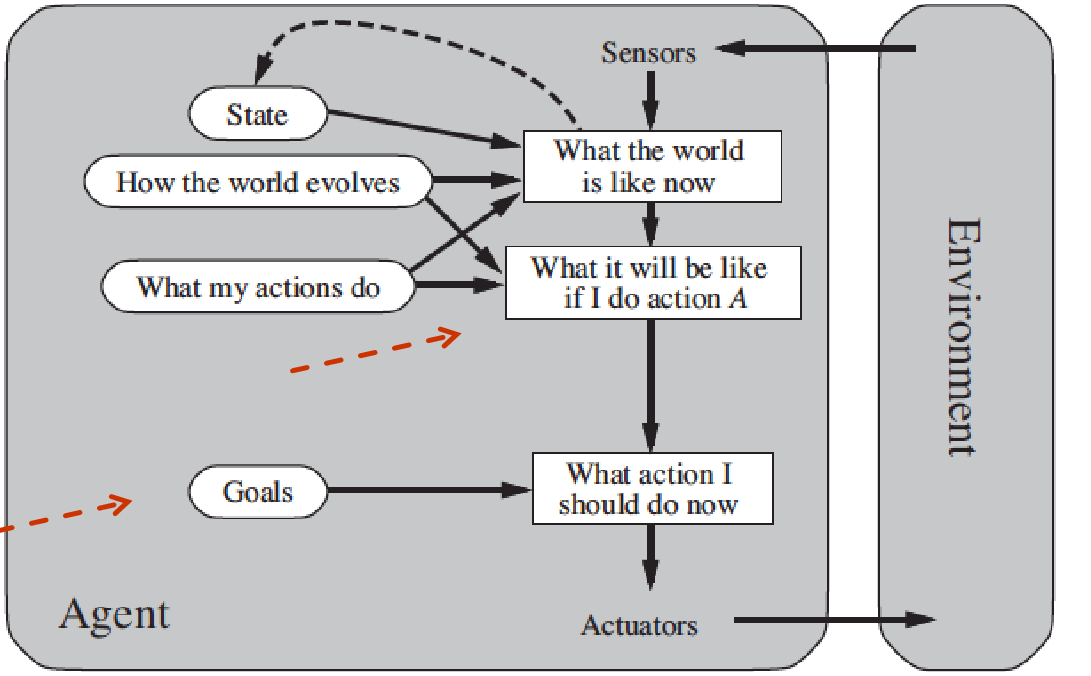
\includegraphics[scale=0.25]{images/agenti_obiettivo.png}
\end{center}

\subsubsection{Agenti con valutazione di utilità}
In questo caso ci sono \textbf{obiettivi alternativi} o più modi per raggiungerlo. L'agente deve quindi decidere verso dove muoversi e si rende necessaria una \textbf{funzione utilità} che associ ad un obiettivo un numero reale. La funzione terrà anche conto della probabilità di successo (\textbf{utilità attesa}).
\begin{center}
	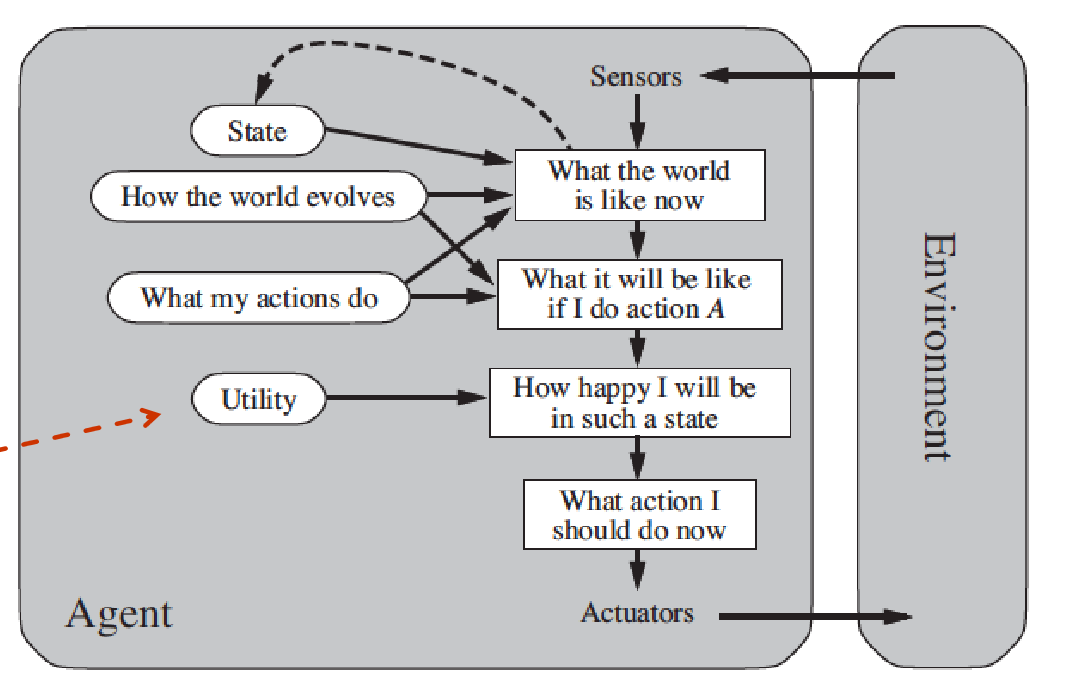
\includegraphics[scale=0.25]{images/agenti_utilita.png}
\end{center}

\subsubsection{Agenti che apprendono}
Questo tipo di agente include la capacità di \textbf{apprendimento} che produce cambiamenti al programma e ne migliora le prestazioni, adattando i comportamenti.\\
L'elemento \textbf{esecutivo} è il programma stesso, quello \textbf{critico} osserva e dà feedback ed infine c'è un generatore di problemi per suggerire nuove situazioni da esplorare.
\begin{center}
	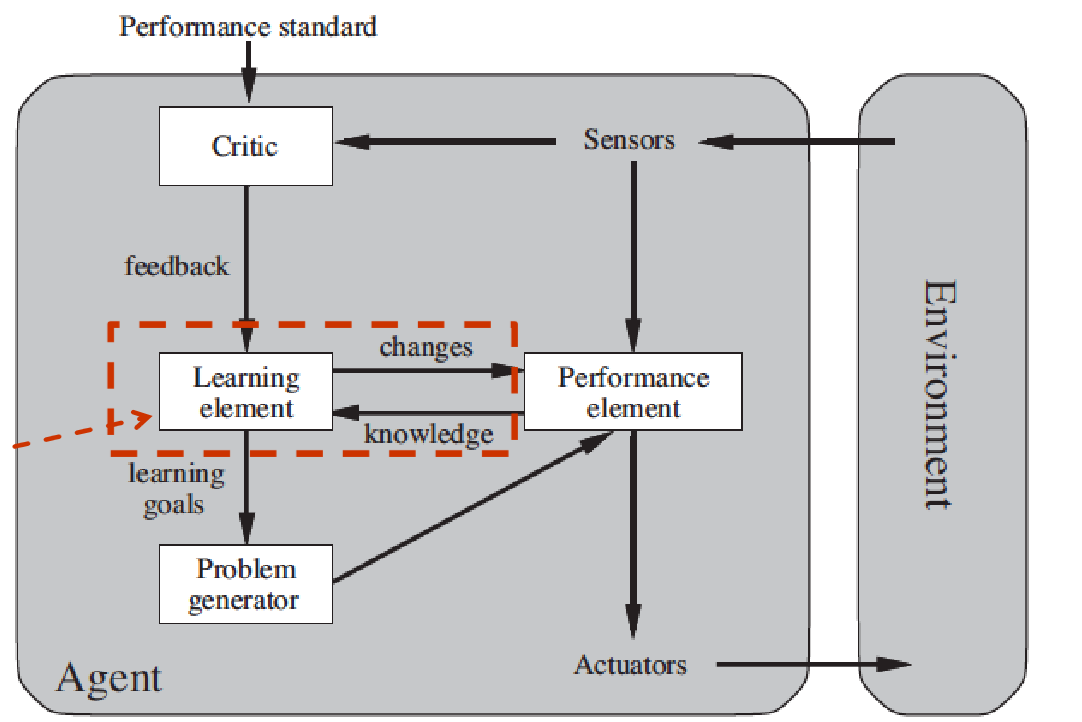
\includegraphics[scale=0.25]{images/agenti_apprendono.png}
\end{center}

\subsubsection{Tipi di rappresentazione}
Gli stati e le transizioni possono essere rappresentati in tre modi:
\begin{itemize}
	\item \textbf{Atomica}: solo con gli stati
	\item \textbf{Fattorizzata}: con più variabili e attributi
	\item \textbf{Strutturata}: con l'aggiunta delle relazioni
\end{itemize}
\begin{center}
	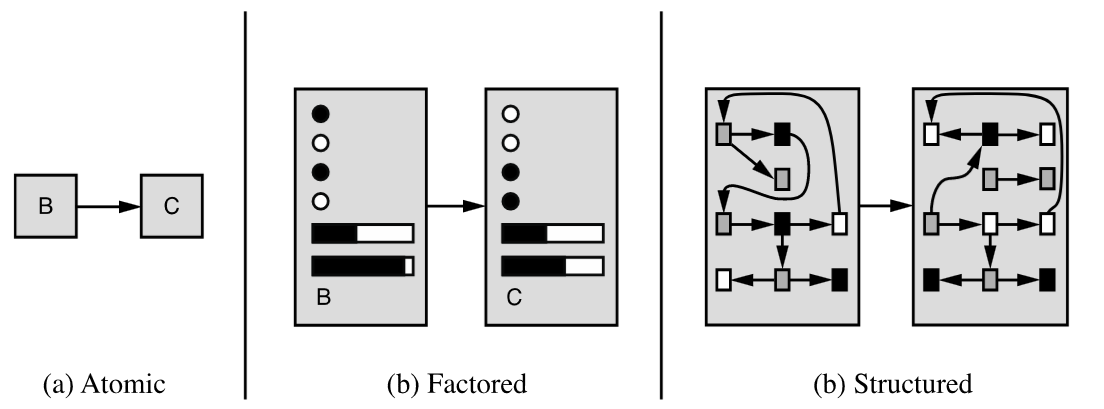
\includegraphics[scale=0.35]{images/rappresentazioni.png}
\end{center}
	% !TeX spellcheck = it_IT
\newpage
\section{Agenti risolutori di problemi}
Gli agenti risolutori di problemi adottano il paradigma della risoluzione di problemi come \textbf{ricerca} in uno \textbf{spazio di stati}. Sono agenti con \textbf{modello} (storia percezioni e stati) che adottano una rappresentazione \textbf{atomica} degli stati.\\
Sono particolari gli agenti con \textbf{obiettivo} che pianificano l'intera sequenza di mosse prima di agire.

\subsection{Processo di risoluzione}
I passi da seguire sono i seguenti:
\begin{enumerate}
	\item \textbf{Determinazione di un obiettivo}, ovvero un insieme di stati in cui l'obiettivo è soddisfatto
	\item \textbf{Formulazione} del problema tramite la rappresentazione degli stati e delle azioni
	\item Determinazione della \textbf{soluzione} mediante la ricerca
	\item \textbf{Esecuzione} del piano
\end{enumerate}

\begin{example}[Viaggio con mappa]
	Supponiamo di voler fare un viaggio. Il processo di risoluzione sarebbe il seguente:
	\begin{enumerate}
		\item Raggiungere Bucarest
		\item \begin{itemize}
			\item Azioni: guidare da una città all'altra
			\item Stato: città su mappa
		\end{itemize}
	\end{enumerate}
\end{example}

\subsection{Assunzioni}
Assumiamo che l'ambiente in questione sia \textbf{statico}, \textbf{osservabile}, \textbf{discreto} e \textbf{deterministico} (assumiamo un mondo ideale).

\subsection{Formulazione del problema}
Un problema può essere definito formalmente mediante 5 componenti:
\begin{enumerate}
	\item \textbf{Stato iniziale}
	\item \textbf{Azioni} possibili
	\item \textbf{Modello di transizione}: $ris: stato \times azione \to stato$, uno stato \emph{successore} $ris(s,a)=s'$
	\item \textbf{Test obiettivo} per capire tramite un insieme di stati obiettivo se il goal è raggiunto $test: stato \to \{true,false\}$
	\item \textbf{Costo del cammino}: composto dalla somma dei costi delle azioni, dove un passo ha costo $c(s,a,s')$. Un passo non ha mai costo negativo.
\end{enumerate}
I punti 1, 2 e 3 definiscono implicitamente lo \textbf{spazio degli stati}. Definirlo esplicitamente può essere molto costoso.

\subsection{Algoritmo di ricerca}
Gli algoritmi di ricerca prendono in input un problema e restituiscono un \textbf{cammino soluzione}.\\
Dobbiamo misurare le \textbf{prestazioni}: trova una soluzione? Quanto costa trovarla? Quanto è efficiente?
\begin{equation*}
	costo\_totale=costo\_ricerca+costo\_cammino\_sol
\end{equation*}

\begin{example}[Arrivare a Bucarest]
	Partiamo con la formulazione del problema:
	\begin{enumerate}
		\item \textbf{Stato iniziale}: la città di partenza, ovvero Arad
		\item \textbf{Azioni}: spostarsi in una città collegata vicina
		\begin{lstlisting}
			Azioni(In(Arad))={Go(Sibiu),Go(Zerind),...}
		\end{lstlisting}
		\item \textbf{Modello di transizione}: 
		\begin{lstlisting}
			Risultato(In(Arad), Go(Sibiu)) = In(Sibiu)
		\end{lstlisting}
		\item \textbf{Test obiettivo}:
		\begin{lstlisting}
			{In(Bucarest)}
		\end{lstlisting}
		\item \textbf{Costo del cammino}: somma delle lunghezze delle strade
	\end{enumerate}
	In questo esempio lo spazio degli stati coincide con la rete dei collegamenti tra le città.
	\begin{center}
		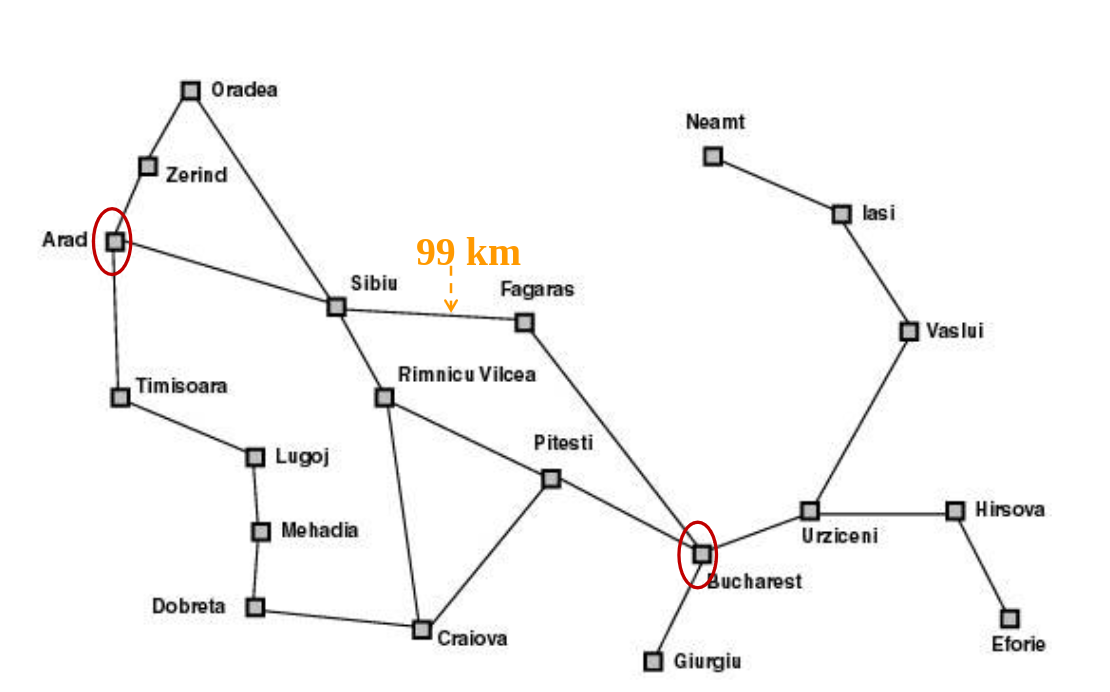
\includegraphics[scale=0.2]{bucarest_example.png}
	\end{center}
\end{example}

\begin{example}[Puzzle dell'8]
	Partiamo con la formulazione del problema:
	\begin{enumerate}
		\item \textbf{Stati}: tutte le possibili configurazioni della scacchiera
		\item \textbf{Stato iniziale}: una configurazione tra quelle possibili
		\item \textbf{Obiettivo}: una configurazione del tipo
		\begin{center}
			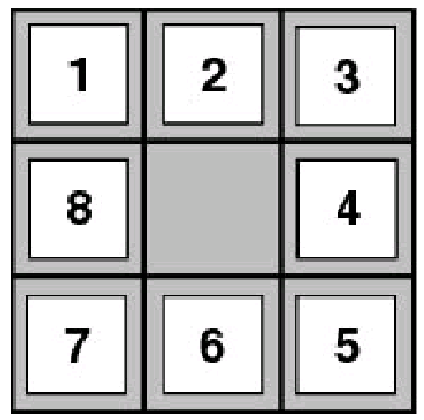
\includegraphics[scale=0.2]{8_puzzle_win.png}
		\end{center}
		\item \textbf{Azioni}: le mosse della casella vuota
		\item \textbf{Costo cammino}: ogni passo costa 1
	\end{enumerate}
	In questo esempio lo spazio degli stati è un grafo con possibili cicli (ci possiamo ritrovare in configurazioni già viste). Il problema è NP-completo: per 8 tasselli ci sono $\frac{9!}{2}=181.000$ stati.
\end{example}

\begin{example}[8 regine]
	Supponiamo di dover collocare 8 regine su una scacchiera in modo tale che nessuna regina sia attaccata da altre.
	\begin{enumerate}
		\item \textbf{Stati}: tutte le possibili configurazioni della scacchiera con 0-8 regine
		\item \textbf{Goal test}: avere 8 regine sulla scacchiera, di cui nessuna è attaccata
		\item \textbf{Azioni}: aggiungi una regina
	\end{enumerate}
	In questo esempio lo spazio degli stati sono le possibili scacchiere, ovvero $64 \times 63 \times \ldots \times 57 \simeq 1.8 \times 10^{14}$.\\
	Proviamo ad utilizzare una formulazione diversa:
	\begin{enumerate}
		\item \textbf{Stati}: tutte le possibili configurazioni della scacchiera in cui \emph{nessuna regina è minacciata}
		\item \textbf{Goal test}: avere 8 regine sulla scacchiera, di cui nessuna è attaccata
		\item \textbf{Azioni}: aggiungere una regina nella colonna vuota più a destra ancora libera in modo che non sia minacciata
	\end{enumerate}
	Lo spazio degli stati passa a $2057$, anche se comunque rimane esponenziale per $k$ regine.\\
	Vediamo infine un'ultima formulazione:
	\begin{enumerate}
		\item \textbf{Stati}: scacchiere con 8 regine, una per colonna
		\item \textbf{Goal test}: nessuna delle regine già presenti è attaccata
		\item \textbf{Azioni}: sposta una regina nella colonna se minacciata
		\item \textbf{Costo cammino}: zero
	\end{enumerate}
	Qui lo spazio degli stati è di qualche decina di milione.\\
	Capiamo quindi che formulazioni diverse del problema portano a spazi di stati di dimensioni diverse.
\end{example}

\begin{example}[Dimostrazione di teoremi]
	Dato un insieme di premesse:
	\begin{equation}
		\{s, t, q \Rightarrow p, r \Rightarrow p, v \Rightarrow q, t \Rightarrow r, s \Rightarrow v\}
	\end{equation}
	dimostrare una proposizione $p$ utilizzando solamente la regola di inferenza \emph{Modus Ponens}:
	\begin{equation*}
		(p \wedge p\Rightarrow q) \Rightarrow q
	\end{equation*}
	Scriviamo la formulazione del problema:
	\begin{itemize}
		\item \textbf{Stati}: insieme di proposizioni
		\item \textbf{Stato iniziale}: le premesse
		\item \textbf{Stato obiettivo}: un insieme di proposizioni contenente il teorema da dimostrare
		\item \textbf{Operatori}: l'applicazione del Modus Ponens
	\end{itemize}
	Lo spazio degli stati è quindi il seguente:
	\begin{center}
		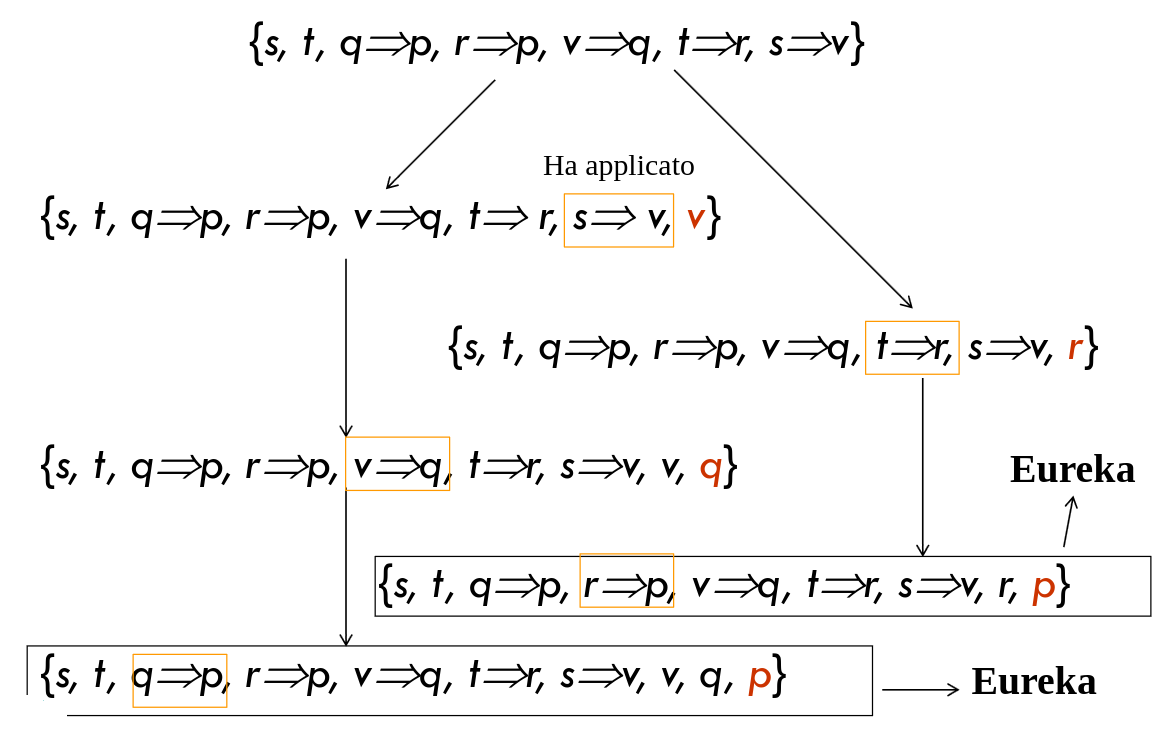
\includegraphics[scale=0.3]{dimostrazione_teoremi.png}
	\end{center}
\end{example}

%TODO Spostare da qui in poi in un altro file
\subsection{Ricerca della soluzione}
La ricerca della soluzione consiste nella generazione di un \textbf{albero di ricerca} a partire dalle possibili sequenze di azioni che si sovrappone allo spazio degli stati.\\
Ad esempio per il caso di Bucarest:
\begin{center}
	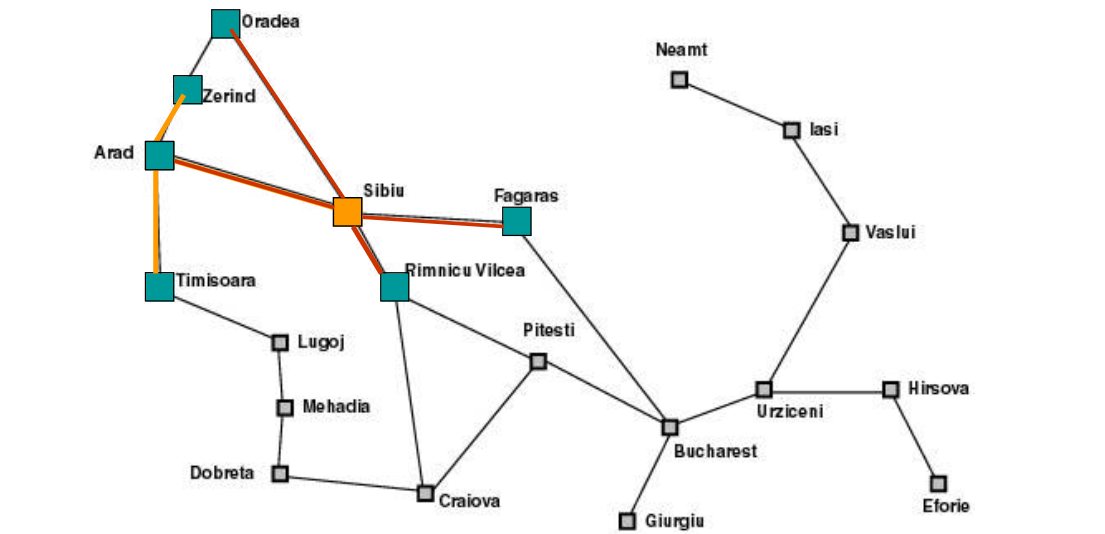
\includegraphics[scale=0.3]{bucarest_tree.png}
\end{center}
Espandiamo ogni nodo con i suoi possibili successori (frontiera).
\begin{definition}[Frontiera]
	Lista dei nodi in attesa di essere espansi (le foglie dell'albero di ricerca).
\end{definition}
\begin{observation}
	Si noti che un nodo dell'albero è diverso da uno stato. Infatti possono esitere nodi dell'albero di ricerca con lo stesso stato (si può tornare indietro).
\end{observation}

\subsection{Strategie di ricerca}
Ci sono diversi tipi di strategia per la ricerca della soluzione:
\begin{itemize}
	\item \textbf{FIFO}
	\item \textbf{LIFO}
	\item \textbf{Coda con priorità}
\end{itemize}

%TODO Ti sei perso delle slide

\subsubsection{Breadth First}
Come esplorare il grafo dello spazio degli stati a livelli progressivi di stessa profondità.\\
Per ogni nodo lo espandiamo, analizziamo i suoi figli (senza scendere ulteriormente di livello) e dopo averli fatti tutti scende di livello seguendo il principio FIFO.\\
Il seguente è il codice della \textbf{ricerca ad albero}, ovvero dove non si torna su un nodo già visitato.

\begin{lstlisting}
	function Ricerca-Ampiezza-A
		returns soluzione oppure fallimento
		nodo = un nodo con stato il problema.stato-iniziale e costo-di-cammino=0
		if problema.Test-Obiettivo(nodo.Stato) then return Soluzione(nodo)
		frontiera = una coda FIFO con nodo come unico elemento
	loop do
		if Vuota?(frontiera) then return fallimento
		nodo = POP(frontiera)
		for each azione in problema.Azioni(nodo.Stato) do
		figlio = Nodo-Figlio(problema, nodo, azione) [costruttore: vedi AIMA]
		if Problema.TestObiettivo(figlio.Stato) then return Soluzione(figlio)
		frontiera = Inserisci(figlio, frontiera) /* frontiera gestita come coda FIFO
	end
\end{lstlisting}

Il seguente è invece quello della \textbf{ricerca su grafo}:
\begin{lstlisting}
	function Ricerca-Ampiezza-g
		returns soluzione oppure fallimento
		nodo = un nodo con stato il problema.stato-iniziale e costo-di-cammino=0
		if problema.Test-Obiettivo(nodo.Stato) then return Soluzione(nodo)
		frontiera = una coda FIFO con nodo come unico elemento
		esplorati = insieme vuoto
	loop do
		if Vuota?(frontiera) then return fallimento
		nodo = POP(frontiera); aggiungi nodo.Stato a esplorati
		for each azione in problema.Azioni(nodo.Stato) do
		figlio = Nodo-Figlio(problema, nodo, azione)
		if figlio.Stato non e in esplorati e non in frontiera then
		if Problema.TestObiettivo(figlio.Stato) then return Soluzione(figlio)
		frontiera = Inserisci(figlio, frontiera) /* in coda
	end
\end{lstlisting}

\noindent Analizziamone la complessità partendo dalle seguenti assunzioni:
\begin{itemize}
	\item Fattore di \textbf{branching} $b$: numero massimo di successori
	\item \textbf{Depth} del nodo obiettivo più superficiale
	\item Lunghezza \textbf{massima} dei cammini nello spazio degli stati
\end{itemize}
La strategia è ottimale se tutti gli operatori hanno lo stesso costo $k$, ovvero se $g(n)=k \cdot depth(n)$, dove $g(n)$ è il costo del cammino per arrivare ad $n$.\\
La complessità nel \emph{tempo} (nodi generati) sarà 
\begin{equation*}
	T(b,d)=1+b+b^2+\ldots+b^d \longrightarrow O(b^d)
\end{equation*}
mentre in \emph{spazio} (nodi in memoria):
\begin{equation*}
	O(b^d)
\end{equation*}
È chiaro che l'algoritmo scali male, sopratutto per quanto riguarda lo spazio.

\subsubsection{Depth first}
In questo algoritmo si parte da un nodo e si scende nel primo figlio, procedendo appunto in profondità. Arrivati alle foglie si torna indietro ai figli precedentemente non visitati. In memoria tengo solamente  i fratelli del path corrente ed elimino i rami già esplorati.\\  Possono esserci tre versioni possibili:
\begin{itemize}
	\item \textbf{Albero}: data $m$ la lunghezza massima dei cammini nello spazio degli stati e $b$ il fattore di diramazione, la \textbf{complessità} in \emph{tempo} è $O(b^m)$ (può essere maggiore di $O(b^d)$) mentre in \emph{spazio} è $b \cdot m$.
	Rispetto al Breadth First, non è né completo né ottimale, ma ci garantisce un notevole risparmio in memoria
	\item \textbf{Grafo}: la memoria corrisponde a tutti i possibili stati, diventando quindi completo nello spazio finito (non in quello infinito)
	\item \textbf{Ricorsiva}: ancora più efficiente per la memoria perché mantiene solo il cammino corrente ($O(m)$). Viene realizzata con un algoritmo di \emph{backtracing} che salva lo stato su uno stack a cui torna in caso di fallimento.
\end{itemize}
\newpage
\begin{lstlisting}
	function Ricerca-DF-A (problema)
		returns soluzione oppure fallimento
		return Ricerca-DF-ricorsiva(CreaNodo(problema.Stato-iniziale), problema)
	
	function Ricerca-DF-ricorsiva(nodo, problema)
		returns soluzione oppure fallimento
		if problema.TestObiettivo(nodo.Stato) then return Soluzione(nodo)
		else
		for each azione in problema.Azioni(nodo.Stato) do
			figlio = Nodo-Figlio(problema, nodo, azione)
			risultato = Ricerca-DF-ricorsiva(figlio, problema)
			if risultato != fallimento then return risultato
		return fallimento
\end{lstlisting}
\subsubsection{Depth Limited}
La ricerca in profondità limitata arriva fino ad un dato livello $l$. È completa solo se si conosce il limite superiore $d$ per la profondità della soluzione e $d<l$. Non è ottimale e ha complessità in tempo $O(b^l)$ e in spazio $O(b \cdot l)$
\subsubsection{Iterative Depth}
Questo approccio prevede di provare l'algoritmo depth limited con limite di profondità $l=0, 1, \ldots$ fino a trovare la soluzione. È il miglior compromesso tra breadth first e depth first:
\begin{itemize}
	\item Complessità in \textbf{tempo} $O(b^d)$ se ammette soluzione
	\item Complessità in \textbf{spazio} $O(b \cdot d)$ se ammette soluzione
\end{itemize}
Quindi ha la \emph{completezza} e l'\emph{ottimalità} del breadth first e la complessità in \emph{spazio} della depth first.
\subsubsection{Uniform Cost}
Partendo da una ricerca in ampiezza, la generalizziamo: si sceglie il nodo di costo minore sulla frontiera e si espande sui contorni di costo uguale.
\begin{center}
	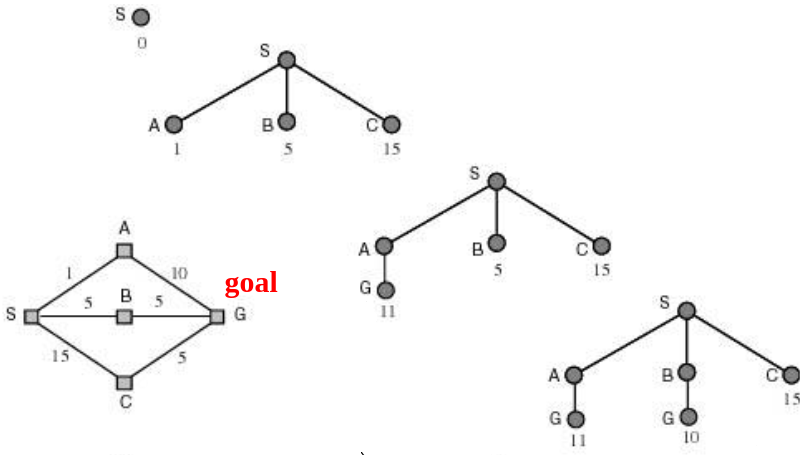
\includegraphics[scale=0.4]{uc.png}
\end{center}
\newpage
Codice per la ricerca su albero:
\begin{lstlisting}
	function Ricerca-UC-A (problema)
			returns soluzione oppure fallimento
			nodo = un nodo con stato il problema.stato-iniziale e costo-di-cammino=0
			frontiera = una coda con priorita con nodo come unico elemento
		loop do
			if Vuota?(frontiera) then return fallimento
			nodo = POP(frontiera)
			if problema.TestObiettivo(nodo.Stato) then return Soluzione(nodo)
			for each azione in problema.Azioni(nodo.Stato) do
				figlio = Nodo-Figlio(problema, nodo, azione)
				frontiera = Inserisci(figlio, frontiera) /* in coda con priorita*/
	end
\end{lstlisting}
Codice per la ricerca su grafo:
\begin{lstlisting}
	function Ricerca-UC-G (problema)
			returns soluzione oppure fallimento
			nodo = un nodo con stato il problema.stato-iniziale e costo-di-cammino=0
			frontiera = una coda con priorita con nodo come unico elemento
			esplorati = insieme vuoto
		loop do
			if Vuota?(frontiera) then return fallimento
			nodo = POP(frontiera);
			if problema.TestObiettivo(nodo.Stato) then return Soluzione(nodo)
			aggiungi nodo.Stato a esplorati
			for each azione in problema.Azioni(nodo.Stato) do
				figlio = Nodo-Figlio(problema, nodo, azione)
				if figlio.Stato non in esplorati e non in frontiera then
					frontiera = Inserisci(figlio, frontiera) /* in coda con priorita
				else if figlio.Stato in frontiera con Costo-cammino piu alto then
					sostituisci quel nodo frontiera con figlio */
	end
\end{lstlisting}
Questo algoritmo è \textbf{ottimo} e \textbf{completo} purché il costo degli archi sia $\epsilon > 0$. Assunto $C^*$ come costo della soluzione ottima, $\lfloor \frac{C^*}{\epsilon}\rfloor$ è il numero di mosse nel caso peggiore. La complessità è quindi $O(b^{1+\lfloor \frac{C^*}{\epsilon}\rfloor})$.
\begin{note}
	Quando ogni azione ha lo stesso costo, la complessità si avvicina a quella della breadth first: $O(b^{1+d})$.
\end{note}
\subsection{Direzione}
Un problema importante è quello della \textbf{direzione} della ricerca, che può essere:
\begin{itemize}
	\item In \textbf{avanti} o guidata da \emph{dati}: si esplora lo spazio di ricerca dallo stato iniziale all'obiettivo
	\item All'\textbf{indietro} o guidata dall'\emph{obiettivo}: si esplora lo spazio di ricerca partendo da uno stato goal e riconducendosi ad un sotto-goal fino a trovare uno stato iniziale
\end{itemize}
Per scegliere la direzione bisogna tenere in conto di quale ha il \textbf{fattore di diramazione} minore.  Si preferisce la ricerca all'\emph{indietro} quando l'obiettivo è ben definito (e.g. theorem proving) mentre quella in \emph{avanti} quando ci sono molteplici obiettivi (e.g. design).\\
\subsubsection{Ricerca bidirezionale}
Nella ricerca bidirezionale si procede in entrambe le direzioni fino ad incontrarsi. La \textbf{complessità} è:
\begin{itemize}
	\item \emph{Tempo}: $O(\sqrt{b^d})$ assumendo che il test dell'intersezione delle due direzioni sia costante
	\item \emph{Spazio}: $O(\sqrt{b^d})$, poiché almeno tutti i nodi di una direzione saranno in memoria
\end{itemize}
Si noti che non sempre è applicabile, come nel caso in cui i predecessori non siano definiti o ci siano troppi stati obiettivo.

\subsection{Problematiche}
\subsubsection{Cicli}
I cammini ciclici rendono gli alberi di ricerca \emph{infiniti} anche quando lo spazio degli stati è finito.
\begin{center}
	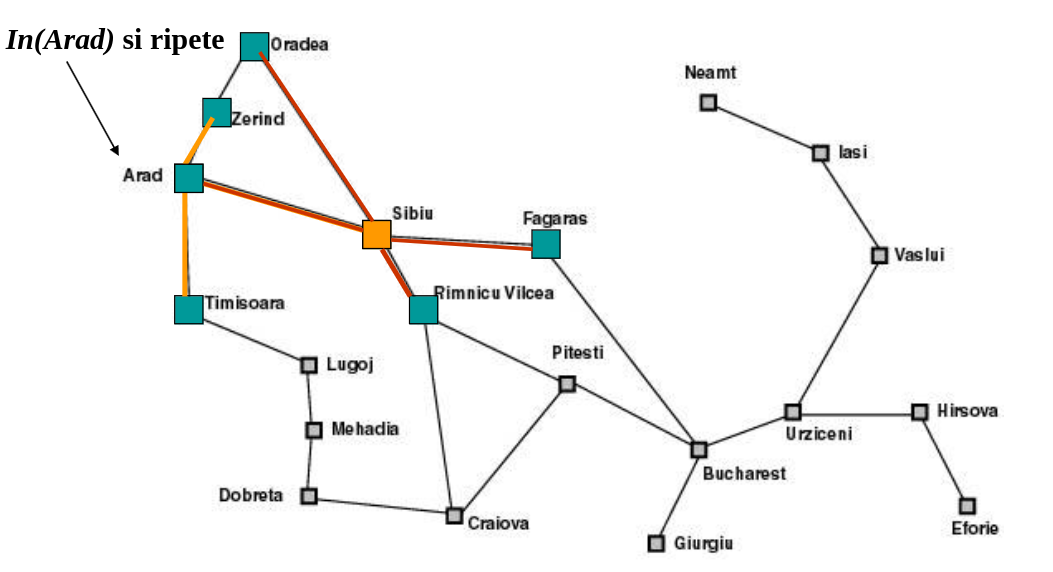
\includegraphics[scale=0.4]{cicli.png}
\end{center}
\subsubsection{Ridondanze}
Su spazi di stati a grafo si possono generare più volte nodi con lo stesso stato nella ricerca, anche in assenza di cicli.
\begin{center}
	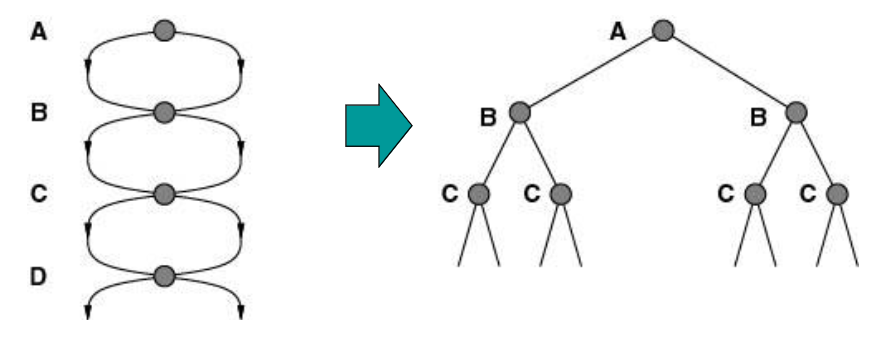
\includegraphics[scale=0.4]{ridondanze.png}
\end{center}
Visitare questi stati è lavoro inutile. Per evitarlo serve \textbf{ricordare} gli stati già visitati, occupando ovviamente più spazio. Tre possibili soluzioni sono:
\begin{enumerate}
	\item Non tornare nel nodo \textbf{genitore}, eliminandolo dai successori (non evita i cammini ridondanti)
	\item Per evitare i \textbf{cammini ciclici} si controlla che  i successori non siano antenati del nodo corrente
	\item Non generare nodi con \textbf{stati già esplorati}: ogni nodo visitato deve essere salvato in memoria
\end{enumerate}
Il costo può essere alto, ad esempio nella depth first la complessità in spazio torna ad essere pari a tutti gli stati.\\
La \textbf{ricerca} sul grafo avverrà quindi come segue:
\begin{enumerate}
	\item Mantiene una lista di stati esplorati (lista chiusa)
	\item Prima di espandere un nodo si controlla se era già stato incontrato o se è già nella frontiera
	\item In quel caso, non viene espanso
\end{enumerate}
Questa tecnica è ottimale solo se abbiamo la garanzia che il costo del nuovo cammino sia maggiore o uguale, ovvero non convenga.
\subsection{Confronto}
\begin{table}[!h]
	\centering
	\begin{tabular}{|c|c|c|c|c|c|c|}
		\hline
		\textbf{Confronto} & \textbf{BF} & \textbf{UC} & \textbf{DF} & \textbf{DL} & \textbf{ID} & \textbf{BDir}\\
		\hline
		Completa & Si & Si(*) & No & Si(**) & Si & Si(***)\\
		Tempo &$O(b^d)$ &$O(b^{1+\lfloor \frac{C^*}{\epsilon}\rfloor})$ & $O(b^m)$ & $O(b^l)$ & $O(b^d)$ & $O(\sqrt{b^d})$ \\
		Spazio &$O(b^d)$ &$O(b^{1+\lfloor \frac{C^*}{\epsilon}\rfloor})$ & $O(b\cdot m)$ & $O(b\cdot l)$ & $O(b\cdot d)$ & $O(\sqrt{b^d})$\\
		Ottimale & Si(****) & Si(*)& No & No & Si(****)& Si(***)\\
		\hline
	\end{tabular}
\end{table}
Legenda:
\begin{itemize}
	\item  \textbf{*}: se $\text{costo archi} \geq \epsilon \geq 0$
	\item \textbf{**}:  se si conosce il limite alla profondità della soluzione ($l>d$)
	\item \textbf{***}: se si utilizza UC o BF
	\item \textbf{****}: se gli archi hanno tutti lo stesso costo
\end{itemize}

	\newpage
\section{Ricerca euristica}
La ricerca esaustiva non è praticabile in problemi di complesità esponenziale (e.g. $10^{120}$ configurazioni in scacchi). Noi usiamo
conoscenza del problemi es esperienza per riconoscere i cammini più promettenti, usiamo una stima del costo futuro, evitando di generare gli altri.
La conoscenza euristica (dal greco "eureka") aiuta fare scelte "oculate", questa ovviamente però non evita la ricerca ma la riduce, consente in
genere di trovare una buona soluzione in tempi accettabilili sotto certe condizioni garantisce completezza e ottimalità.\\\\
La conoscenza del problema data tramite una funzione di valutazione $f$, che include $h$ detta \textbf{funzione di valutazione euristica}.
$$h: n \to R$$
La funzione si applica al nodo ma dipende solo dallo stato (n.Stato).
\begin{note}
    Manteniamo la notazione in $n$ per unifomritò con $g$; $g$ dipende anche dal cammino fino al nodo.
\end{note}
$$f(n) = g(n) + h(n) \text{ove g(n) è il costo cammino visto con UC}$$
Per procedere preferibilmente verso il percorso migliore, seguendo problem-specific information, di stima del costo futuro:
\begin{itemize}
    \item La città più vicina (o la città più vicina alla metà in linea d'aria - tabella esterna) nel problema dell'itinerario.
    \item Il numero della caselle fuori posto nel gioco dell'otto.
    \item Il vataggio in pezzi della dama o negli scacchi
\end{itemize}

\begin{example}
    Mappa Romania dist. in linea d'aria.
    \begin{figure}[h!]
        \centering
        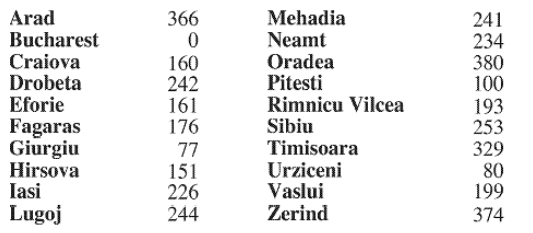
\includegraphics[width=0.75\textwidth]{images/esempio-euristica-h.png}
    \end{figure}
\end{example}

\subsection{Algoritmo di ricerca Best-first}
Il \textbf{best first - heuristic} usa lo stesso algoritmo di UC \footnote{Warning: AIMA ed. IV ha usato uno schema di
UC diverso e alcune proprietà cambiano} ma con uso di $f$ (stima di costo) per la coda con priorità.
Una volta scelta $f$ determina la strategia di ricerca. A ogni passo si sceglie il nodo sulla frontiera per cui il valore della $f$ è 
migliore (il nodo più promettente).
\begin{note}
    Migliore significa "minore" in caso di un'euristica che stima la distanza della soluzione
\end{note}
\hspace{-15pt}Un caso speciale: \textbf{greedy best-first}, su usa solo $h (f=h)$.
\begin{example}
    Esempio di greedy best-first con $f=h$
    \begin{figure}[h!]
        \centering
        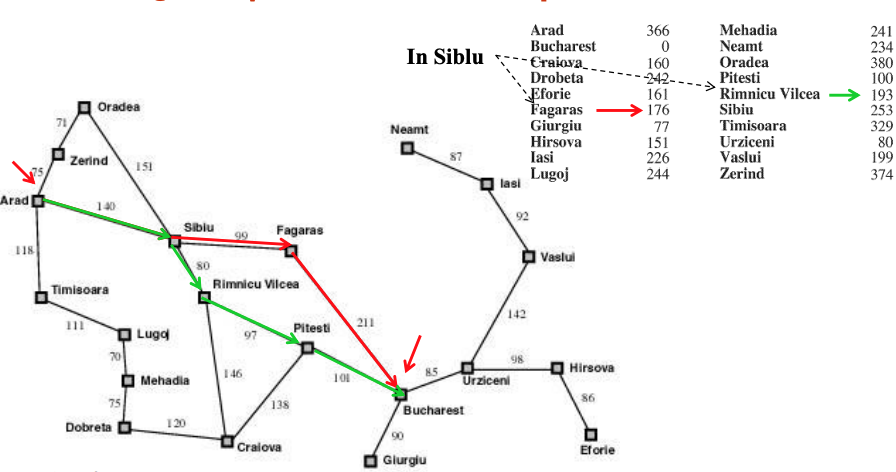
\includegraphics[width=0.75\textwidth]{images/esempio-best-first.png}
    \end{figure}
    Da Arad a Bucarest con \textbf{Greedy best-first}: Arad, sibiu, fagaras, bucharest (450) ma non è l'ottimale
    che sarebbe: Arad, Sibiu, Rimnicu, Pitesti, Bucarest (418).
\end{example}

\subsection{Algoritmo A}
Si può dire qualcosa di $f$ per avere garanzie di completezza e ottmialità?
\begin{definition}
    Un \textbf{Algoritmo A} è un algoritmo di best first con una fuzine di valutazione dello stato del tipo:
    $$f(n) = g(n) + h(n) \:\: \text{con}\:\: h(n) \geq 0 \:\: \text{e}\:\: h(goal) = 0$$
\end{definition}
In questa definizione abbiamo che $g(n)$ è il costo del cammino percorso per raggiugnere n, mentre $h(n)$ una
stima del costo per raggiungere da n un nodo goal (distanza).\\
Vedremo alcuni casi particolari dell'algoritmo A:
\begin{itemize}
    \item Se $h(n) = 0 \:\:[f(n) = g(n)]$ si ha \textbf{Ricerca Uniforme (UC)}.
    \item Se $g(n) = 0 \:\:[f(n) = h(n)]$ si ha \textbf{Greedy Best First}.
\end{itemize}
\begin{example}
    Esempio nel gioco dell'otto.
    \begin{figure}[h!]
        \centering
        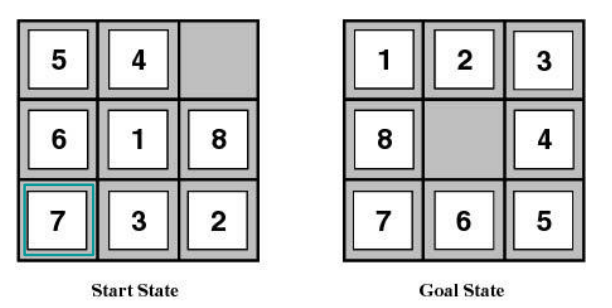
\includegraphics[width=0.6\textwidth]{images/esempio-gioco-otto.png}
    \end{figure}

    \hspace{-15pt}$f(n) = \#\text{mosse fatte} \:\: + \:\: \#\text{caselle-fuori-posto} \hspace{10pt} f(start) = 0 + 7 \hspace{10pt} f(goal-state) = ? + 0$\\
    Dopo $\leftarrow, \downarrow, \uparrow, \rightarrow$ abbiamo che $f = 4 + 7$, stesso stato, $g$ è cambiato.
\end{example}
\begin{theorem}
    L'algoritmo A con la condizione:
    $$g(n) \geq d(n) \cdot \epsilon \hspace{10pt}(\epsilon >0 \text{ costo minimo arco})$$
    è completo (con $d(n)$ che è la distanza).
\end{theorem}
\begin{note}
    La conzione ci garantisce che non si verifichino situazioni strane del tipo:
    \begin{figure}[h!]
        \centering
        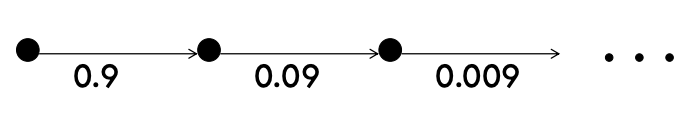
\includegraphics[width=0.65\textwidth]{images/nota-alg-completo.png}
    \end{figure}
    e quindi che il costo lungo un cammino non cresca "abbastanza" (se cresce abbastanza possiamo fermare quel path per costo alto di g).
\end{note}
\begin{demostration}
    Sia $[n_0, n_1, n_2, \dots, n', \dots, n_k = goal]$ un cammino soluzione. Sia $n'$ un nodo della frontiera su un cammino soluzione:
    $n'$ prima o poi sarà espanso. Infatti esistono solo un numero finito di nodi $x$ che possono essere aggiunti alla frontiera con $f(x) \leq f(n')$
    (è la condizione sulla crescita di g, scritta precedentemetne, tale che non esista una catena infinita di archi e nodi che possa aggiungere con costo sempre $\leq f(n')$).\\\\
    Quindi, se non si trova una soluzione prima, $n'$ verrà espanso e i suoi successori aggiunti alla frontiera. Tra questi anche il suo successore sul cammino soluzione.\\
    Il ragionamento si può ripetere fino a dimostrare che anche il nodo goal sarà selezionato per l'espanzione.
\end{demostration}

\subsection{Algoritmo $A^*$}
La funzione di valutazione ideale (oracolo):
$$f^*(n) = g^*(n) + h^*(n)$$
Con $g^*(n)$ il costo del cammino minimo da radice a n, $h^*(n)$ costo del cammino minimo da n a goal, $f^*(n)$ costo
del cammino minimo da radice a goal, attraverso n. Normalmente:
$$g(n) \geq g^*(n) \hspace{10pt} e \hspace{10pt} h(n) \text{ è una stima di } h^*(n)$$
($g(n) \geq g^*(n)$ rappresenta costo cammino $\geq$ costo migliore). Si può andare in sottostima (e.g. linea d'aria) o 
sovrastima della distanza dalla soluzione.
\begin{definition}[Euristica ammissibile]
    $$\forall n\:\: t.c.\:\: h(n) \leq h^*(n) \:\:\:\: \text{h è una sottostima}$$
\end{definition}
\begin{example}
    L'euristica della distanza in linea d'aria.
\end{example}
\begin{definition}[Algoritmo $A^*$]
    Un algoritmo A in cui h è una funzione euristica ammissibile.
\end{definition}
\begin{theorem}
    Gli algoritmi $A^*$ sono \textbf{ottimali}.
\end{theorem}
\begin{corollaries}
    $BF^{(+)}$ e UC sono ottimali ($h(n) = 0$).
\end{corollaries}
\begin{example}
    Itinerario con $A^*$ (ad albero).
    \begin{figure}[h!]
        \centering
        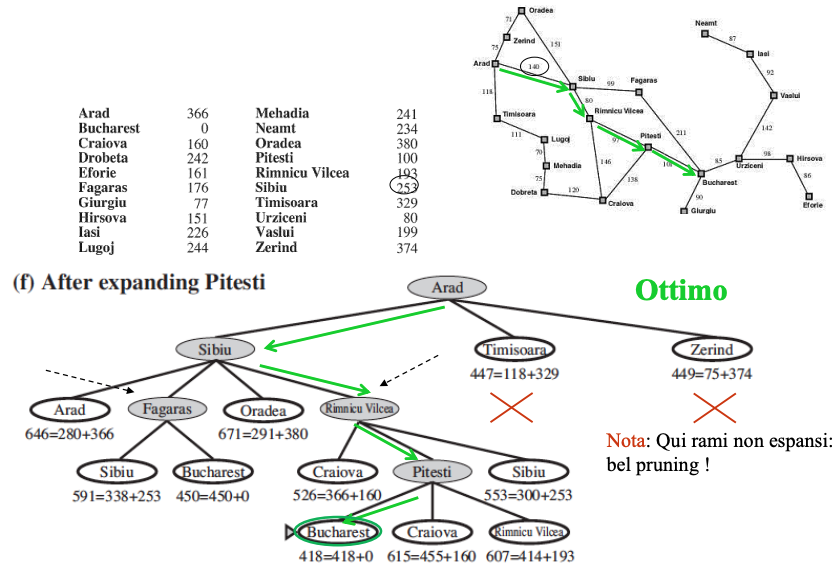
\includegraphics[width=0.62\textwidth]{images/itinerario-A*-albero.png}
    \end{figure}
\end{example}
\begin{observation}
    Alcune osservazioni su $A^*$
    \begin{enumerate}
        \item Rispetto a greedy best-first, la componente g fa si che si abbandonino cammini che vanno troppo in profondità.
        \item Ha sotto o sovra stima?
        \begin{enumerate}
            \item Una sottostima (h) può farci compiere del lavoro inutile (tenendo anche candidati non buoni), però non ci 
            fa perdere il cammino migliore (quando prendo nodo goal è il cammino migliore).
            \item Una funzione che qualche volta sovrastima può farci perdere la soluzione ottimale (taglio per causa di sovrastima, invece era buona)
        \end{enumerate}
    \end{enumerate}
\end{observation}

\subsubsection{Ottimalità su $A^*$}
\begin{wrapfigure}[8]{r}{5cm}
    \vspace{-30pt}
    \centering
    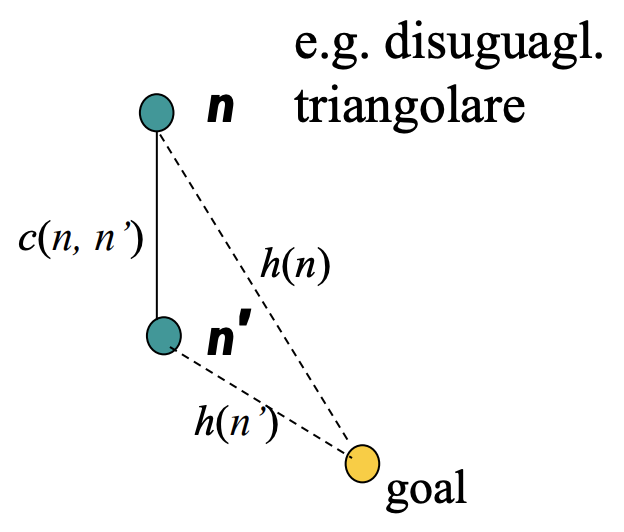
\includegraphics[width=4cm]{images/dis-triagolare.png}
\end{wrapfigure}
Nel caso di ricerca a/su albero l'uso di un'euristica ammissibile è sufficente a garantire l'ottimalità su $A^*$.
Nel caso di ricerca su grafo (con UC come visto) serve una proprietà più forte: la \textbf{consistenza} (detta anche \textbf{monotonicità}).\\\\
Per evitare rischio di scartare candidati ottimi (stato già incontrato) si vuol evitare, causa uso della lista esplorati, di far sparire, o meglio
non considerare al momento dell'espansione, candidati ottimali. Cerchiamo quindi condizioni per garantire che il primo espanso sia il migliore.

\begin{definition} 
    Un euristica \textbf{consistente} $[h(goal) = 0]$ (consistenza locale).
    $$\forall n \:\: t.c. \:\: h(n) \leq c(n, a, n') + h(n') \text{ dove n' è un successore di n}$$
\end{definition}
\hspace{-15pt}Ne segue che $f(n) \leq f(n')$
\begin{note}
    Se h è consistente la $f$ non decresce mai lungo i cammini, da cui il termine \textbf{monotona}.
\end{note}
\begin{theorem}
    Un'euristica monotona è ammissibile.
\end{theorem}
\hspace{-15pt}Esistono euristiche ammissibili che non sono monotone, ma sono rare. Le euristiche monotone garantiscino che la soluzione meno costosa 
venga trovata per rima e quindi sono ottimali anche nel caso di ricerca su grafo.\\
Non si devono recuperare tra gli antenati nodi con costo minore. Lista degli esplorati, stato già esplorato è sul cammino ottimo allora posso
evitare di inserire il corrente ripetuto senza perdere l'ottimalità.
\begin{lstlisting}
    if figlio.Stato non e in esplorati e non e in frontiera then
        frontiera = Inserisci(figlio, frontiera)
\end{lstlisting}
Per la frontiera, volendo evitare stati ripetuti, resta 'if' finale di UC:
\begin{lstlisting}
    if figlio.Stato e in frontiera con Costo-cammino piu alto then
        sostituisci quel nodo frontiera con figlio 
\end{lstlisting}
Andiamo ora a verificare l'ottimalità di $A^*$ supponendo di avere il teorema, con $h$ consistente.
\begin{enumerate}
    \item Se $h(n)$ è consistente i valori di $f(n)$ lungo un cammino sono non decrescenti:
    $$\text{se } h(n) \leq c(n, a, n') + h(n') \hspace{10pt} \Rightarrow \text{(def. consistenza sommando g(n))}\hspace{10pt} g(n) + h(n) \leq g(n) + c(n, a, n') + h(n')$$
    ma siccome abbiamo $g(n) + c(n, a, n') = g(n')$ allora
    $$g(n) + h(n) \leq g(n') + h(n') \Rightarrow f(n) \leq f(n') \Rightarrow f \text{ monotona}$$
    \item Ogni volta che $A^*$ seleziona un nodo (n) per l'espansione, il cammino ottimo a tale nodo è stato trovato: 
    se così non fosse, ci sarebbe un altro nodo m ella frontiera sul cammino ottimo (a n, ancora da trovare con un cammino ottimo), con $f(m)$
    minore (per la monotonia e n successore di m); ma ciò non è possibile perché tale nodo sarebbe già stato espanso (si espande prima un nodo con f minore).
    \item Quando seleziona nodo goal è cammino ottimo $[h=0, f=C^*]$.
\end{enumerate}
% TODO: AGGIUNGI IMMAGINI
Quindi, detto questo, perché $A^*$ è vantaggioso?
\begin{itemize}
    \item $A^*$ espande tutti i nodi con $f(n) < C^*$ ($C^*$ = costo ottimo)
    \item $A^*$ espande alcuni nodi con $f(n) = C^*$.
    \item \textbf{$A^*$ non espande alcun nodo con $f(n) > C^*$}
\end{itemize}
Quindi alcuni nodi (e suoi sottoalberi) non verranno considerati per l’ espansione (ma restiamo ottimali):
pruning (h opportuna, più alta possibile tra le ammissibili, fa tagliare molto).\\\\
% TODO: AGGIUNGI IMMAGINE
Più f è aderente a stima ottimale, più taglio! Ovali più stretti. Cercheremo quindi una h il più alta possibile tra le ammissibili
Se molto bassa molti (sino a tutti i) nodi restano minore di $C^* \to$ espando tutti (a cerchi).
Il pruning sotto-alberi è il punto focale: non li abbiamo già in memoria e evitiamo di generarli (decisivo per i problemi di AI a spazio stati esponenziali.\\\\
In riassunto L’algoritmo è quello degli schemi usati per UC, Usando f = g+h per la coda con priorità, ove h e g soddisfano quanto allo slide 9 [A], 
ove h è una funzione euristica ammissibile $[A^*]$, e considerando le condizioni dette per ottenere l’ottimalità su grafi.
\begin{itemize}
    \item $A^*$ è \textbf{completo}: discende dalla completezza di A ($A^*$ è un algoritmo A particolare).
    \item $A^*$ con euristica monotona è \textbf{ottimale}.
    \item $A^*$ è \textbf{ottimamente efficiente}: a parità di euristica nessn altro algoritmo espande meno nodi (senza rinunciare a ottimalità)
\end{itemize}
I problemi principali sono la scelta dell'euristica e  ancora l'occupazione di memoria che nel caso
pessimo resta esponenziale come visto per gli altri algoritmi di ricerca con stesso schema, causa frontiera.

\subsection{Sotto-casi speciali: US e Greedy Best First}
Ci sono due casi particolai dell'algoritmo A:
\begin{enumerate}
    \item Se $h(n) = 0$ $[f(n) = g(n)]$ si ha Uniform Cost (UC), ossia $g$ non basta (si può migliorare).
    \item Se $g(n) = 0$ $[f(n) = h(n)]$ si ha Greedy Best Fist, ossia $h$ non basta (già visto all'inizio).
\end{enumerate}
\subsubsection{UC vs $A^*$}
Illustrazione dell'algoritmo di ricerca Dijkstra per trovare il percorso da un nodo iniziale (in basso
sinistra, rosso) a un nodo obiettivo (in alto a destra, verde) in un problema di pianificazione del movimento del robot.
I nodi aperti rappresentano l'insieme "provvisorio". I nodi pieni sono quelli visitati, con colore
che rappresenta la distanza: più verde, più lontano. Nodi in tutti i diversi
le direzioni vengono esplorate in modo uniforme, apparendo come un fronte d'onda più o meno circolare
poiché l'algoritmo di Dijkstra utilizza un'\textbf{euristica identicamente uguale a 0}. $\to$ UC !\\\\
\begin{wrapfigure}[6]{r}{5cm}
    \vspace{-35pt}
    \centering
    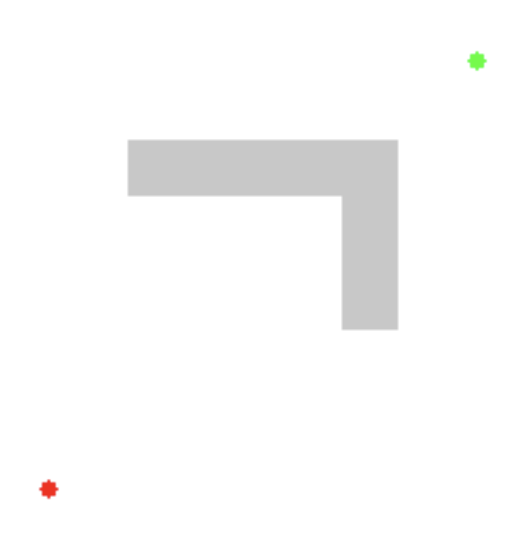
\includegraphics[width=3cm]{images/dijkstra.png}
\end{wrapfigure}
Illustrazione dell'algoritmo di ricerca A* per trovare il percorso da un nodo iniziale a un nodo obiettivo in un robot è un
problema di pianificazione del movimento. I cerchi vuoti rappresentano i nodi nell'insieme aperto, cioè,
quelli che restano da esplorare e quelli pieni sono nell'insieme chiuso. Colore acceso
ogni nodo chiuso indica la distanza dalla partenza: più è verde, più è lontano. Uno
può prima vedere A* muoversi in linea retta in direzione della porta, poi quando colpisce l'ostacolo, esplora percorsi alternativi attraverso i nodi da insieme aperto $\to$ frontiera.\\\\
L'algoritmo A* è una generalizzazione dell'algoritmo di Dijkstra che riduce le dimensioni del sottografo che deve essere esplorato, se il lower-bound
della "distanza" dall'obiettivo (h) è disponibile.

\subsection{Costruire le euristiche di $A^*$}
Partiamo dalle valutazione di funzioni euristiche. A parità di ammissibilità, una euristica può essere più
efficiente di un’altra nel trovare il cammino soluzione migliore (visitare meno nodi). Questo dipende da quanto
informata è l'euristia (dal \textbf{grado di informazione posseduto}) 
\begin{itemize}
    \item $h(n) = 0$ minimo di informazione (BF o UC)
    \item $h^*(n)$ massimo di infomrazione (oracolo)
\end{itemize}
In generale, per le euristiche ammissibili:
$$0 \leq h(n) \leq h^*(n)$$
\begin{theorem}
    Se $h_1 \leq h_2$, i nodi espansi\footnote{Ricorda che $A^*$ espande tutti i nodi con $f(n) = g(n) + h(n) < C^*$, e sono meno per $h$ maggiore (h maggiore fa andare più nodi oltre $C^*$).} da $A^*$ con $h_2$ sono un sottoinsieme di quelli espandi da $A^*$ con $h_1$.
\end{theorem}
\hspace{-15pt}Se $h_1 \leq h_2$, $A^*$ con $h_2$ è almeno efficiente quanto $A^*$ con $h_1$.
Un’euristica più informata (accurata) riduce lo spazio di ricerca (è più efficiente), ma è tipicamente più costosa da calcolare (e.g. un caso estremo ?)
\begin{example}
    Due euristiche ammissibili per il gioco dell'8 potrebbero essere le seguenti:
    \begin{itemize}
        \item $h_1$: conta il numero di caselle fuori posto
        \item $h_2$: somma delle distanze \textbf{Manhattan} (orizzonatle/verticale) delle caselle fuori posto dalla posizione finale.
    \end{itemize}
    $h_2$ è più informata di $h_1$, infatti $\forall n \:\:.\:\: h_1(n) \leq h_2(n)$, quindi si dice che $h_2$ \textbf{domina} $h_1$ (utile per confrontte tra ammissibili)
    \begin{figure}[h!]
        \centering
        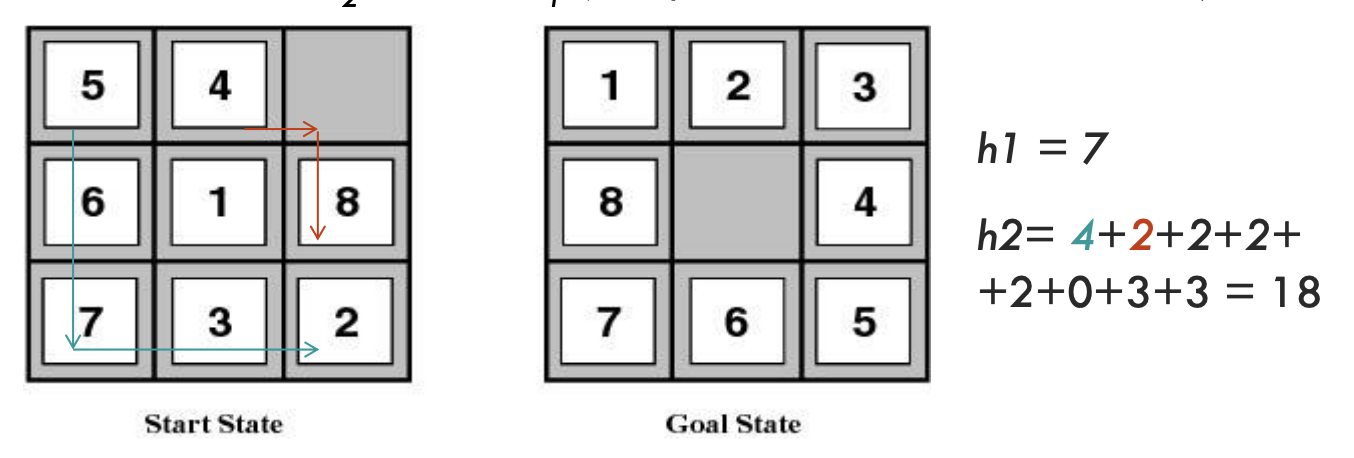
\includegraphics[width=0.65\textwidth]{images/euristica-gioco-8.png}
    \end{figure}
\end{example}
\begin{definition}
    La somma delle distanze Manghattan si definisce come:
    $$h((x,y)) = MD((x,y), (x_g, y_g)) = |x - x_g| + |y - y_g|$$
\end{definition}
\begin{figure}[h!]
    \centering
    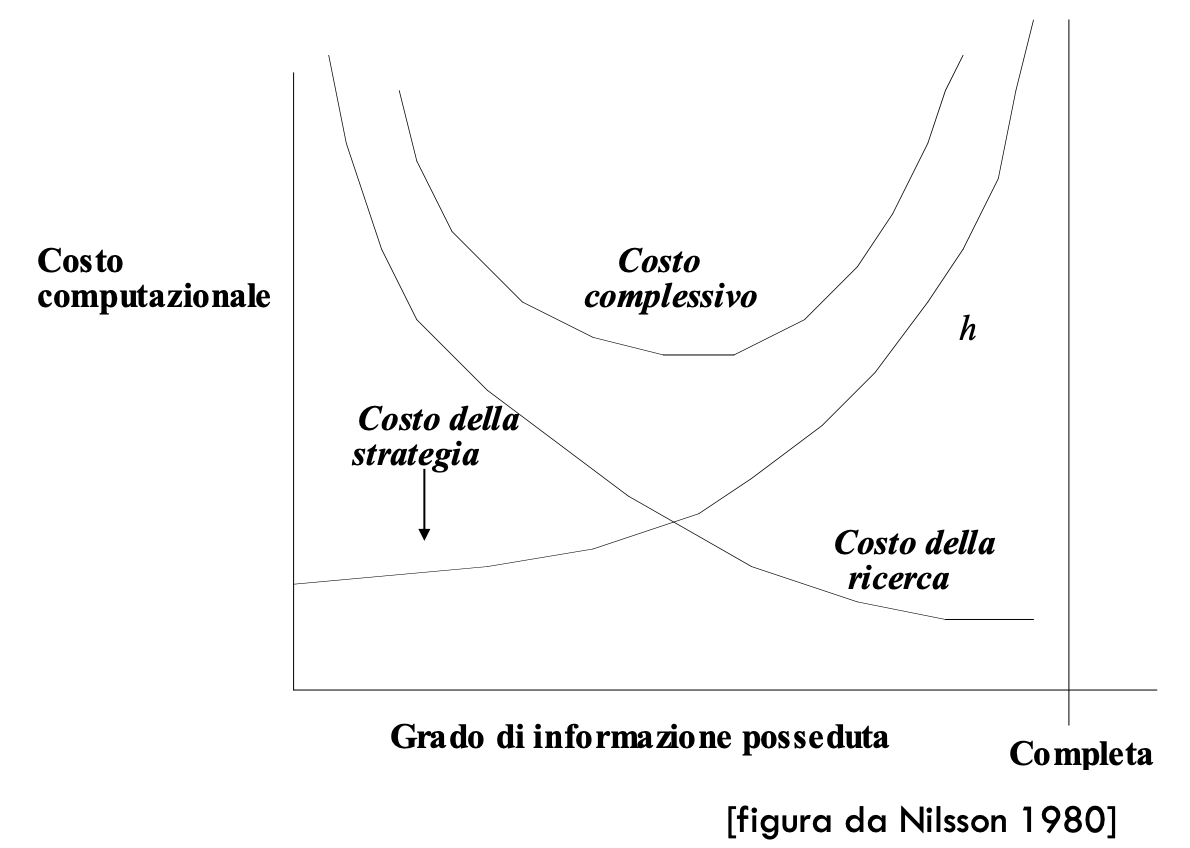
\includegraphics[width=0.60\textwidth]{images/costo-ricerva-vs-costo-euristica.png}
    \caption{Costo ricerca vs costo euristico}
\end{figure}
\hspace{-15pt}Ora capiamo come valutare gli algoritmi di ricerca euristica. Introfuciamo
il \textbf{fattore di diramazione effettivo} $b^*$, N: numero di nodi generati, d: profondità della soluzione.
$b^*$ è il fattore di diramazione di un albero uniforme con $N+1$ nodi, solizione dell'equazione:
$$N + 1 = b^* + (b^*)^2 + \dots + (b^*)^d$$
Sperimentalmente una buona euristica ha un $b^*$ abbastanza vicino a 1 (<1.5)
\begin{example}
    Ricodando l'esempio dal gioco dell'otto:
    \begin{figure}[h!]
        \centering
        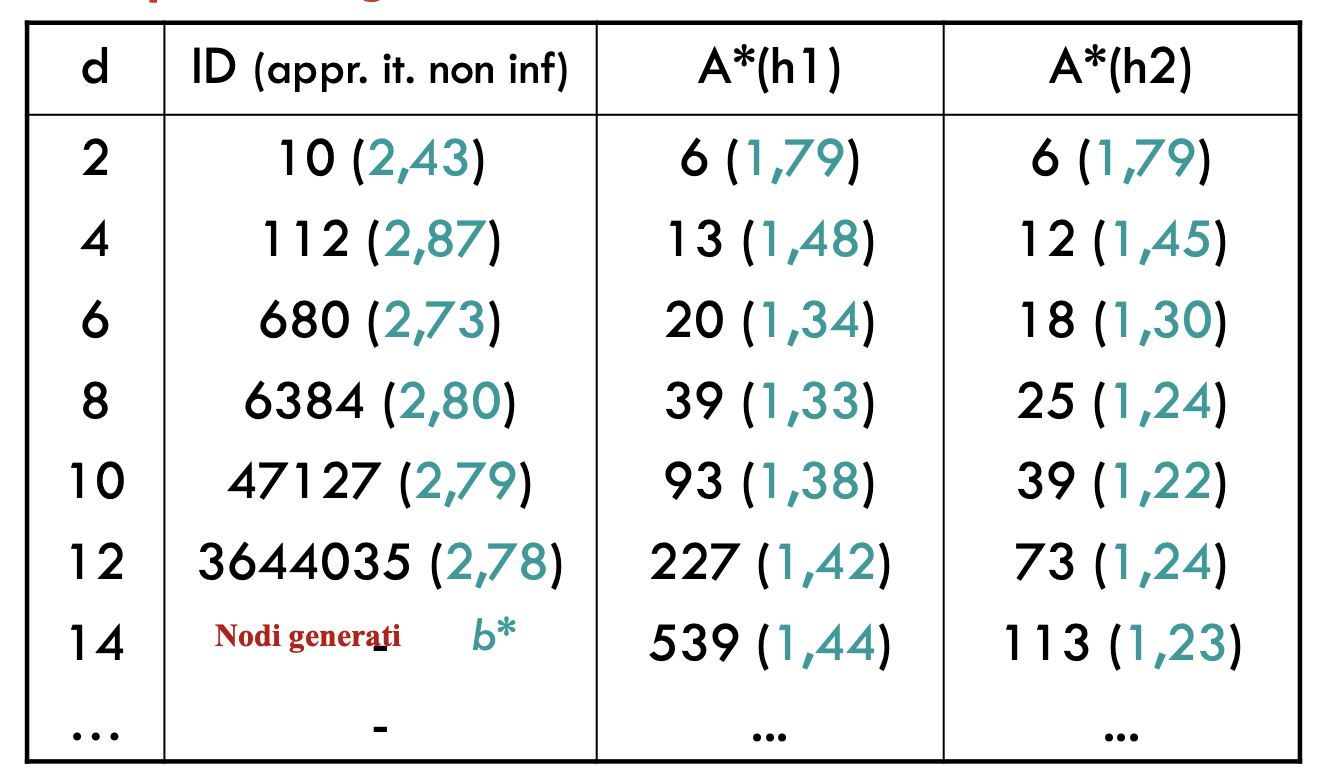
\includegraphics[width=0.60\textwidth]{images/gioco-otto-misura-euristiche.png}
    \end{figure}
    Sono riportati: Nodi generati e fattore di diramazione effettivo ($b^*$, verde)
    I dati sono mediati, per ogni d, su 100 istanze del problema [AIMA].\\\\
    Nella \textbf{capacità di esplorazione}, l'influenza di $b^*$:
    \begin{itemize}
        \item Con b=2: d=6 e N = 100 \hspace{15pt} d=12 e N = 10.0000
        \item Con b=1.5: d=12 N = 100 \hspace{15pt} d=24 e N = 10.000
    \end{itemize}
    migliorando di poco l’euristica si riesce, a parità di nodi espansi, a raggiungere una profondità doppia di esplorazione mosse!
\end{example}

\subsection{Inventare euristiche}
Quindi abbiamo che:
\begin{enumerate}
    \item Tutti i problemi dell’IA (o quasi) sono di complessità esponenziale ... (nel generare nodi, i.e. configurazioni possibili) ma c’è esponenziale e esponenziale!
    \item L’euristica può migliorare di molto la capacità di esplorazione dello spazio degli stati rispetto alla ricerca cieca.
    \item Migliorando anche di poco l’euristica si riesce ad esplorare uno spazio molto più grande (più in profondità).
\end{enumerate}
Per inventare un euristica ci sono alcune strategie, che aiutano appunto ad ottenre euristiche amissibili:
\begin{itemize}
    \item Rilassamento del problema
    \item Massimizzazione di euristiche
    \item Database di pattern disgiunti
    \item Combinazione lineare
    \item Apprendere dall’esperienza
\end{itemize} 
\subsubsection{Rillassamento problema}
\begin{example}
    Il rilassamento del problema nel gioco dell’8 mossa da A a B possibile se: 
    \begin{enumerate}
        \item \textbf{B adiacente a A}
        \item \textbf{B libera}
    \end{enumerate}
    $h_1$ e $h_2$ sono calcoli distanza esatta della soluzione in versioni semplificate del puzzle:
    \begin{itemize}
        \item $h_1$ (nessuna restrizione, ne 1 ne 2): sono sempre ammessi scambi a piacimento tra caselle (si muove
        ovunque) $\to$ numero caselle fuori posto.
        \item  $h_2$ (solo restrizione 1): sono ammessi spostamenti anche su caselle occupate, purché adiacenti $\to$ somma delle distanze Manhattan.
    \end{itemize}
\end{example}

\subsubsection{Massimizzazione di euristiche}
Se si hanno una serie di euristiche ammissibili $h_1, h_2, \dots, h_k$ \textbf{senza che nessuna "domini" un'altra}
allora conviene prendere il massimo dei lori valori:
$$h(n) = max(h_1(n), h_2(n), \dots, h_k(n))$$
Se le $h_i$ sono ammissibili, anche la $h$ lo è. La h domina tutte le altre.

\subsubsection{Database con pattern disgiunti}
\begin{figure}[h!]
    \centering
    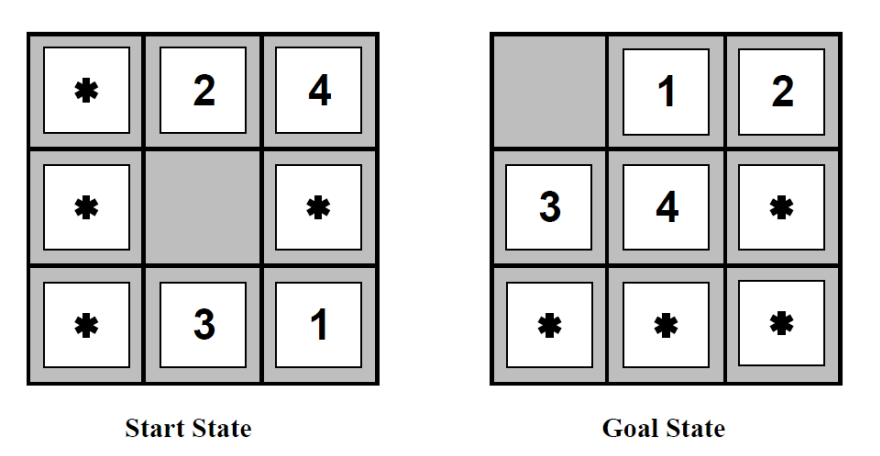
\includegraphics[width=0.65\textwidth]{images/euristiche-da-sottoproblemi.png}
\end{figure}
\hspace{-15pt}Costo della soluzione ottima al sottoproblema (di sistemare 1,2,3,4) è una sottostima del costo per il problema nel suo
complesso (e.g. rilevatesi più accurata della Manhattan). \\
\textbf{Database di pattern}: memorizzare ogni istanza del
sottoproblema con relativo costo della soluzione. Usare poi questo database per calcolare $h_{DB}$ (estraendo dal DB la
configurazione corrispondente allo stato completo corrente).
\begin{itemize}
    \item \textbf{Domanda}: Potremmo poi fare la stessa cosa per altri sottoproblemi: 5-6-7-8, 2-4-6-8, ottenendo altre euristiche ammissibili,
    poi prendere il valore massimo: ancora una euristica ammissibile. Ma potremmo sommarle e ottenere un’euristica
    ancora più accurata?
    \item \textbf{Risposta}: In generale no perché le soluzioni ai sottoproblemi interferiscono (condividono alcune mosse, se sposto 1-2-3-4, spostero
    anche 4-5-6-7) e la somma delle euristiche in generale non è ammissibile (potremmo sovrastimare avendo avuto aiuti mutui).
    Si deve eliminare il costo delle mosse che contribuiscono all’altro sottoproblema. Database di pattern disgiunti consentono di sommare i
    costi (euristiche additive) [e.g. solo costo mosse su1-2-3-4], sono molto efficaci: gioco del 15 in pochi ms
    ma per esempio difficile scomporre per cubo Rubik.
\end{itemize}

\subsubsection{Apprendimento dall'esperienza}
Bisogna eseguire un apprendimento dall'esperienza. Quindi far girare il programma, raccogliere dati: coppie
$<stato, h^*>$. Usare i dati per apprendere a predire la h con algoritmi di apprendimento induttivo (da istanze note stimiamo h in generale).\\
Gli algoritmi di apprendimento si concentrano su caratteristiche salienti dello stato (feature, xi) [e.g.
apprendiamo che da numero tasselli fuori posto 5 $\to$ costo~14, etc].

\subsubsection{Combinazione euristiche}
Quando diverse caratteristiche influenzano la bontà di uno stato, si può usare una combinazione lineare per combinare le euristiche:
$$h(n) = c_1 x_1(n) + c_2x_2(n) + \dots + c_k x_k(n)$$
\begin{example}
    Gioco dell'8: $h(n) = c_1 \:\: \#\text{fuori-posto} + c_2 \#\text{coppie-scambiate}$\\
    Scacchi: $h(n) = c_1 \:\text{vant-pezzi} + c_2 \:\text{pezzi-attacc.} + c_3 \:\text{regina} + \dots$
\end{example}
\hspace{-15pt}Il peso dei coefficienti può essere aggiustato con l’esperienza, anche qui apprendendo automaticamente da esempi di gioco.
$h(goal) = 0$ (e.g. gioco dell’8) ma ammissibilità e consistenza non automatiche.

\subsection{Algoritmi evoluti basati su $A^*$}
Ci sono una serie di algoritmi basati su $A^*$ che possono andare a portare ad un miglioramento dell'occupazione della memoria.
Fra questi abbiamo: Beam search, A* con approfondimento iterativo (IDA*), ricerca best-first ricorsiva (RBFS), A* con memoria limitata (MA*) in versione semplice (SMA*).

\subsubsection{Beam search}
Nel Best First viene tenuta tutta la frontiera; se l’occupazione di memoria è eccessiva si può ricorrere ad una variante: la Beam search.
La Beam Search tiene ad ogni passo solo i k nodi più promettenti, dove k è detto l’ampiezza del raggio
(beam). La Beam Search non è completa.

\subsubsection{IDA${}^*$}
L'$IDA^*$ è un $A^*$ con approfondimento iterativo. IDA* combina A* con ID: ad ogni iterazione si ricerca
in profondità con un limite (cut-off) dato dal valore della funzione f (e non dalla profondità) il limite f-limit viene aumentato ad ogni iterazione,
fino a trovare la soluzione. Punto critico: di quanto viene aumentato f-limit.
\begin{example}
    \begin{figure}[h!]
        \centering
        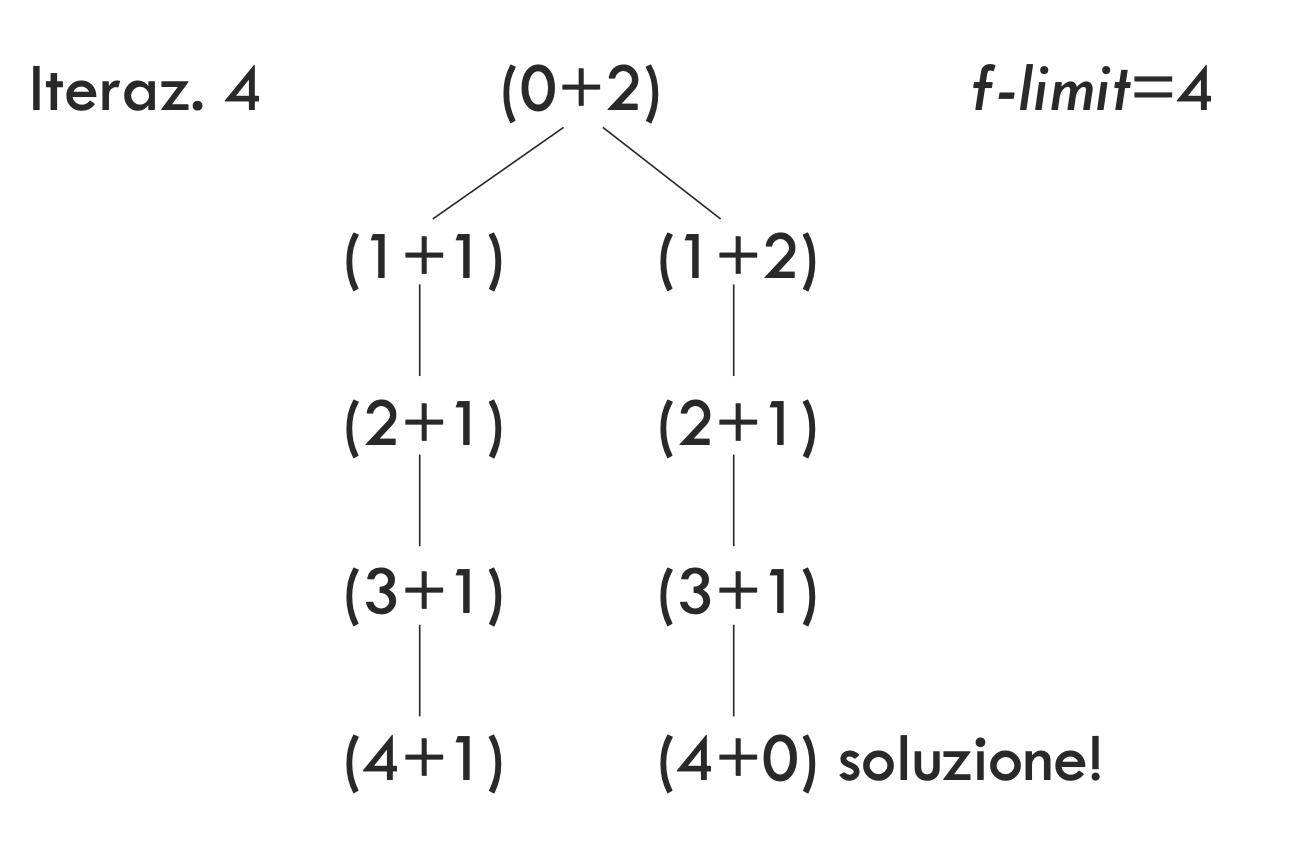
\includegraphics[width=0.65\textwidth]{images/esempio-ida*.png}
    \end{figure}
\end{example}
\hspace{-15pt}Cruciale la scelta dell'incremento per garantire l’ottimalità:
\begin{itemize}
    \item Nel caso di costo delle azioni fisso è chiaro: il limite viene incrementato del costo delle azioni.
    \item Nel caso che i costi delle azioni siano variabili? O costo minimo, oppure si potrebbe ad ogni passo fissare il limite successivo al
    valore minimo delle f scartate (in quanto superavano il limite) all’iterazione precedente.
\end{itemize}
$IDA^*$ è sia completo che ottimale.
\begin{itemize}
    \item Se le azioni hanno costo costante k (caso tipico 1) e f-limit viene incrementato di k.
    \item Se le azioni hanno costo variabile e l'incremento di f-limit è $\leq \epsilon$ (minimo costo degli archi).
    \item Se il nuovo f-limit = min. valore f dei nodi generati ed esclusi all'iterazione precedente.
\end{itemize}
L'occupazione di memoria è $O(bd)$.

\subsubsection{Best-first ricorsivo (BRFS)}
Simile a DF ricorsivo: cerca di usare meno memoria, facendo del lavoro in più. Tiene traccia ad ogni livello del \textbf{migliore percorso
alternativo}. Invece di fare backtracking in caso di fallimento (DF si ferma solo in fondo) interrompe l’esplorazione quando
trova un nodo meno promettente (secondo f). Nel tornare indietro si ricorda il miglior nodo che ha
trovato nel sottoalbero esplorato, per poterci eventualmente tornare Memoria: lineare nella profondita delle sol. ottima.
\begin{example}
    \begin{figure}[h!]
        \centering
        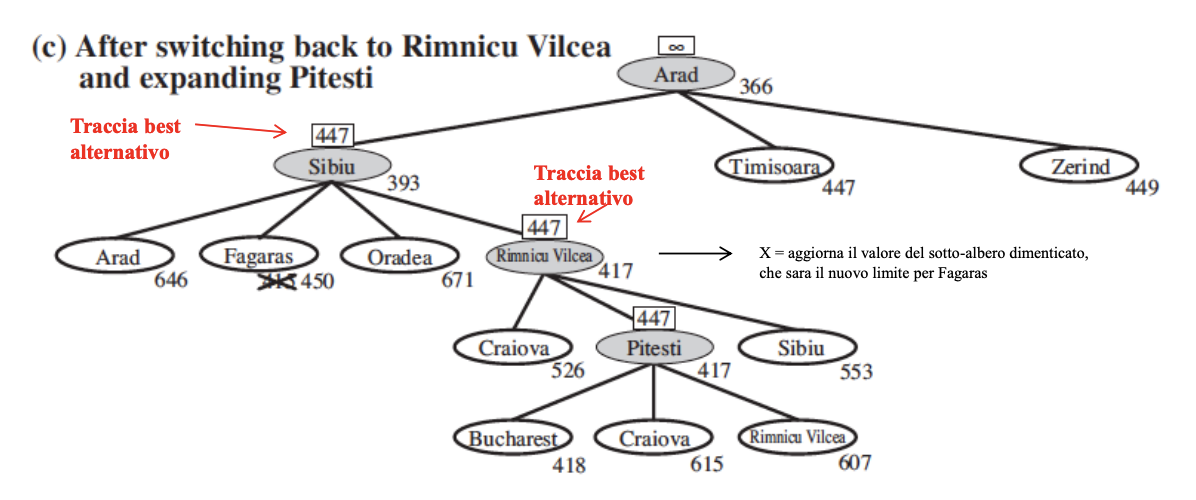
\includegraphics[width=0.65\textwidth]{images/esempio-best-first-ricorsivo.png}
    \end{figure}
\end{example}
\begin{lstlisting}
    function Ricerca-Best-First-Ricorsiva(problema)
        returns soluzione oppure fallimento
        // all inizio f-limite e un valore molto grande
        return RBFS(problema, CreaNodo(problema.Stato-iniziale), infinito) 

    function RBFS (problema, nodo, f-limite)
        // restituisce due valori
        returns soluzione oppure fallimento e un nuovo limite all f-costo 
        if problema.TestObiettivo(nodo.Stato) then return Soluzione(nodo)
        successori = [ ]

        for each azione in problema.Azioni(nodo.Stato) do
            aggiungi Nodo-Figlio(problema, nodo, azione) a successori // genera i successori
        if successori vuoto then return fallimento, infinito

        for each s in successori do // valuta i successori
            s.f = max(s.g + s.h, nodo.f) // un modo per rendere monotona f
        loop do
            migliore = il nodo con f minimo tra i successori
            if migliore.f > f_limite then return fallimento, migliore.f
            alternativa = il secondo nodo con f minimo tra i successori
            risultato, migliore.f = RBFS(problema, migliore, min(f_limite, alternativa))
            if risultato != fallimento then return risultato
\end{lstlisting}

\subsubsection{$A^*$ con memoria limitata (versione semplice)}
L'idea è quella di utilizzare al meglio la memoria disponibile. $SMA^*$ procede come $A^*$ fino ad esaurimento della
memoria disponibile. A questo punto \textbf{“dimentica” il nodo peggiore}, dopo avere aggiornato il valore del padre.
A parità di f si sceglie il nodo migliore più recente e si dimentica il nodo peggiore più vecchio. Ottimale se il cammino soluzione sta in memoria.\\\\
In conclusione in algoritmi a memoria limitata (IDA* e SMA*) le limitazioni della memoria possono portare a compiere
molto lavoro inutile [esp. ripetuta stessi nodi]. Difficile stimare la complessità temporale effettiva. Le limitazioni di memoria possono rendere un problema intrattabile dal punto di vista computazionale.
\end{document}
